\newcounter{descriptcounti}
\newcounter{descriptcountii}
\newlist{enumfunctional}{description}{2}
\setlist[enumfunctional,1]{%
  before={\setcounter{descriptcounti}{0}%
          \renewcommand*\thedescriptcounti{\myprefix\arabic{descriptcounti}}}
  ,font=\bfseries\stepcounter{descriptcounti}\thedescriptcounti~
}
\setlist[enumfunctional,2]{%
  before={\setcounter{descriptcountii}{0}%
          \renewcommand*\thedescriptcountii{\myprefix\arabic{descriptcounti}.\arabic{descriptcountii}}}
  ,font=\bfseries\stepcounter{descriptcountii}\thedescriptcountii~
}

\newlist{enumnonum}{description}{1}
\setlist[enumnonum,1]{%
  before={\setcounter{descriptcounti}{0}%
          \renewcommand*\thedescriptcounti{\myprefix}}
  ,font=\bfseries\stepcounter{descriptcounti}\thedescriptcounti
}

% Do not forget to include Introduction
%---------------------------------------------------------------
% \chapter{Introduction}
% uncomment the following line to create an unnumbered chapter
\chapter*{Úvod}\addcontentsline{toc}{chapter}{Úvod}\markboth{Úvod}{Úvod}
%---------------------------------------------------------------
\setcounter{page}{1}

% The following environment can be used as a mini-introduction for a chapter. Use that any way it pleases you (or comment

\acrshort{iot}, neboli Internet of Things, je trend, který na sebe v posledních letech poutá stále větší pozornost a přibývá potenciálních uživatelů, kteří by chtěli výhod takových zařízení a systémů využívat. Jelikož však díky obrovskému pokroku, který potkal svět IT jako takový v posledních desetiletích, můžeme dnes narazit na zařízení spadající pod označení \enquote{chytré} opravdu na všech místech každodenního života, přibývá také dle očekávání počet výrobců zařízení, standardů pro komunikaci a ovládání, ale také způsobů, jak tyto zařízení vzdáleně ovládat, spravovat a propojovat.

Vzhledem ke skutečnosti, že většina komerčních řešení je vyvíjena za účelem zisku, není překvapením, že výrobci jednotlivých \acrshort{iot} komponent nejsou vždy zaměření na vytvoření kompatibilních celků, které mohou být využívány s komponentami vyráběnými jinými společnostmi, jelikož by tímto krokem často přicházeli o část tržeb. Komunitní řešení, tvořená neziskovými spolky, jsou ale často zbytečně komplikovaná, protože se snaží dosáhnout podpory co největšího počtu spolupracujících částí. Ani nejuniverzálnější z projektů však nenabízí vskutku pravou univerzálnost, jelikož existuje velké množství projektů tvořených na míru, často rukama domácích kutilů nebo malých podnikatelů, kteří svými projekty cílí na podstatně menší skupinu, než je tomu u nadnárodních značek.

Já sám doma využívám zařízení, která mají vlastní způsob komunikace, který nepodléhá žádnému zaběhnutému standardu. Bohužel tak není snadný způsob, jak takové zařízení ovládat pomocí zaběhlých a známých řešení, které jsem popsal dále v této práci, a je potřeba využívat ovládací rozhraní, které vylo vytvořeno na míru k danému zařízení - pokud však vůbec nějaké takové existuje. Proto jsem se rozhodl vytvořit webové rozhraní, které bude sloužit ke správě různých \acrshort{iot} zařízení, jejich ovládání a zjišťování hodnot z jejich stavu a čidel.

I kdyby se mně, nebo jakémukoliv jinému uživateli, podařilo připojit své na míru vytvářené zařízení s unikátním způsobem komunikace k některým dostupným řešením pro správu a ovládání \acrshort{iot} zařízení, byla by opravdu mizivá šance, že by to bylo řešení podporující funkcionalitu, kterou jsem ve svém hledání napříč platformami zatím téměř nenašel, a tou je plánování změny stavu zařízení předem. Tato změna bude provedena automaticky bez zásahu uživatele za předem zadaných podmínek.

Jelikož je oblast \acrshort{iot} mou zálibou ve volném čase a dlouhou dobu se mi nedařilo najít řešení, které jsem já, ale se mnou jistě mnoho dalších uživatelů s podobnými požadavky, vyžadoval, rozhodl jsem se pro vypracování vlastního řešení. Mou motivací je také vyzkoušet si práci na větším projektu, který bude od počátku navrhován pro využití nejen osobní, ale i kýmkoliv ze širší veřejnosti, což se u běžných školních projektů děje zřídkakdy a je třeba u takových projektů dbát na dokumentaci a správný návrh. V neposlední řadě mě také zajímá, zda se mnou zvolené technologie, které nutně nejdou ruku v ruce s trendy v oboru, ukáží jako správná, a třeba i efektivnější volba, než jsou jejich někdy populárnější alternativy.



\chapter*{Cíl práce}\addcontentsline{toc}{chapter}{Cíl práce}\markboth{Cíl práce}{Cíl práce}
%---------------------------------------------------------------
\setcounter{page}{2}

Cílem této práce je vytvořit vlastní implementaci webového rozhraní, pomocí kterého budou moci uživatelé projektu ovládat svá \acrshort{iot} zařízení. Toto rozhraní bude implementováno tak, aby mohlo běžet v několika instancích, které se navzájem nebudou ovlivňovat, a budou ho nejen díky tomu moci uživatelé provozovat pomocí vlastního hardwaru. Zároveň však bude umožňovat dostatečnou separaci uvnitř aplikace pomocí uživatelských účtů a jejich práv, čímž bude umožněno používat jednu instanci webového rozhraní i více skupinami uživatelů, kterým bude zaručeno dostatečné soukromí a oddělení jejich účtů a zařízení od jimi neautentizovaných uživatelů.

Toto rozhraní bude umožňovat správu uživatelských účtů, zařízení, specifikaci jejich komunikačních kanálů, ale také přidávání jednotlivých účtů a zařízení do správních skupin, ve kterých budou uživatelům pomocí přidělení rolí odemykán přístup k různým úrovním přístupu a možnostem úprav.

V práci bude také vytvořen a popsán způsob, jakým bude zajištěno, aby uživatel mohl přidat modul, který \emph{naučí} aplikaci nový způsob, jak komunikovat se zařízením, které neumožňuje komunikaci žádným z dodaných způsobů. Tento modul bude naprogramován a zkompilován uživatelem a přidán do jeho instance aplikace, čímž bude zajištěno, že neovlivní ostatní instance této aplikace, používané jinými uživateli.

Zařízení bude možné ovládat pomocí jednoduchých ovládacích prvků, ke kterým bude mít přístup pouze přihlášený a autentizovaný uživatel. Tyto ovládací prvky budou generovány dynamicky podle charakteristik zařízení. Aplikace bude také implementovat \emph{sekvence}, tedy \emph{posloupnosti kroků} (\emph{krokem} rozumíme odeslání jedné zprávy zařízení serverem). Jednotlivé kroky této sekvence mohou ovládat několik různých zařízení, mohou záviset na některých stavových hodnotách zařízení a mohou být provedeny současně s předchozím krokem, ale také po uběhnutí předem stanovené časové prodlevy od vykonání posledního kroku. Celá sekvence může být spuštěna manuálně uživatelem, ale také naplánována na minutové, hodinové, ale i denní bázi. 

Dalším rozšířením tohoto projektu by poté mohlo být například umožnění spouštění sekvencí na základě jakýchkoliv změn stavu zařízení nebo přidání \emph{lokálních sekvencí}, tedy posloupností příkazů, které by byly prováděny v režii programu běžícího na zařízené lokálně blízkém ovládanému zařízení, umožňující relaxaci jedné z vrstev komunikace mezi serverem a samotným hardwarem.

%---------------------------------------------------------------
\chapter{Průzkum stávajících řešení}
%---------------------------------------------------------------

%---------------------------------------------------------------
\section{Závěrečné práce studentů FIT ČVUT na podobné téma}
%---------------------------------------------------------------

\subsection{Bc. Jakub Vejr - Webové prostředí pro správu a konfiguraci \acrshort{iot} projektů}

V této diplomové práci autor popisuje jím vytvořenou aplikaci, která má za úkol zaznamenávat příchozí data ze senzorů, zpracovávat je, a tyto data a trendy z nich vycházející poté zobrazovat pomocí webového rozhraní. Autor si vybral jako hlavní platformu projektu jazyk JavaScript, přesněji řečeno Node.js a framework Express. Jednotlivá zařízení komunikují s backendovou částí projektu pomocí \acrshort{rest} \acrshort{api}, která poté data rozklíčuje z příchozích souborů a pomocí databáze MongoDB je uchovává. Uživatelé této aplikace jsou rozděleni na správce s možností přidávat uživatele i \acrshort{iot} zařízení, a běžné uživatele, kteří pracují jen s omezenou množinou dat. Frontendová část aplikace je napsaná pomocí Next.js a knihovny React. Aplikace tedy funguje především směrem od zařízení k cílovému uživateli, který nemá možnost své \acrshort{iot} zařízení ovládat. 

\subsection{Bc. Jan Prášil - Webová aplikace pro sběr a zpracování dat \acrshort{iot}}

Diplomová práce pana Prášila popisuje a vytváří aplikaci, která má být na frontendové straně de facto upravenou a personalizovanou úpravou JavaScript knihovny Grafana, která se používá k analýze a zobrazování nejrůznějších typů dat s možností notifikace uživatelů, na backendové straně se poté využívá Node.JS, který provozuje \acrshort{rest} \acrshort{api}, přes který se poté připojuje klientské rozhraní. Backend také komunikuje se službou Microsoft SharePoint Server 2013, což bylo jedním z požadavků při zadávání této práce. Jedná se o podnikovou aplikaci dělanou na míru, díky které mohou uživatelé s pravomocemi v aplikaci rozdělenými dle typu jejich účtu provádět správu \acrshort{iot} zařízení, nebo si zobrazovat údaje z nich získané. Tato aplikace také funguje spíše jako jednosměrný kanál informací.

\subsection{Martin Skalický - \acrshort{iot} platforma s webovým rozhraním}

TODO1

%---------------------------------------------------------------
\section{Existující řešení}
%---------------------------------------------------------------

V dnešní době najdeme na trhu nepřeberné množství produktů, které nám umožní interakci s \acrshort{iot} zařízeními. Pro širší veřejnost jsou pravděpodobně známější produkty od velkých nadnárodních společností, které se nespecializují výhradně na tvorbu \acrshort{iot} platforem, ale tyto produkty vytváří spíše jako přesah svých dalších služeb, jako je například Google Home od společnosti Google, nebo SmartThings od společnosti Samsung. Ty jsou známě především díky skvělé integraci těchto platforem přímo do operačních systémů těch zařízení, které jsou vyráběny právě v koprodukci těchto globálních gigantů. Tento trend ale nepozorujeme pouze u firem populárních na západní části světa, stejnou cestu například zvolila i společnost Xiaomi a její aplikace na správu a ovládání \acrshort{iot} zařízení pojmenovaná Xiaomi Home.

Do další skupiny můžeme zařadit produkty, které jsou vyvíjeny úspěšnými společnostmi, které se specializují na výrobu přímo \acrshort{iot} zařízeních jako takových, a pro snadné propojení svých zařízení mezi sebou vytvořili svou vlastní \acrshort{iot} platformu. Takovými společnostmi jsou například Philips a její Philips Hue, používaný primárně pro ovládání všech typů domácího osvětlení od tohoto výrobce, TP-LINK se svým nově vzniklou řadou produktů Tapo, EVOLVEO a aplikace na správu kamer EVOLVEO CAM.

V průběhu let se ale ukázalo, že omezovat svá zařízení pouze na jedinou, a často totožnou společností produkovanou, možnost, jak je může jejich uživatel ovládat, je z obchodního hlediska nečekaně kontraproduktivní, jelikož pouze minimum zákazníků používá všechna chytrá zařízení vyrobená pouze jednou firmou. Jednotlivé firmy mají totiž často nerovnoměrnou kvalitu i kvantitu možností napříč jednotlivými typy \acrshort{iot} zařízení a proto je pro zákazníka nejpohodlnější koupit si různé výrobky od různých firem. Proto se na trhu staly populárními zařízení podporující několik, a často i konkurenčních, ovládacích aplikací.

V této době začaly vznikat i projekty společností i jednotlivců, které cílí pouze na tvorbu ovládacího softwaru pro co nejvíce typů \acrshort{iot} zařízení napříč výrobci, ale samy zařízení jako takové nevyrábí. Díky oblíbenosti a řádově menším nákladům je těchto projektů v dnešní době dostupných desítky až stovky. Některé z nich jsou dokonce tak populární, že sami výrobci inzerují své \acrshort{iot} zařízení s informací, že podporují ovládaní těmito prostředky. Jejich nevýhodou oproti řešením popsaných výše jsou ale často poplatky za použití, jelikož narozdíl od společností, které svůj výdělek získají z prodeje hardwaru a ovládací software často přikládají zdarma, společnosti bez hardwaru musí získávat peníze na vývoj a údržbu těchto produktů jinými způsoby, a to často právě prodejem přístupu k těmto ovladačům, nebo zpoplatněním některých jejich služeb.

Poslední skupinou jsou opensource projekty, tedy projekty, které mají veřejně dostupný zdrojový kód. Tyto produkty se vyznačují tím, že za nimi často stojí dobrovolnická komunita nadšenců, kteří často projekt vytváří ve svém volném čase, většinou jsou také tyto produkty kompletně zdarma, nebo maximálně s placenými vylepšeními. Mají však ale také své nevýhody, často nejsou tak uživatelsky přívětivé jako placené, komerčně vytvářené alternativy. I přes občasnou menší funkcionalitu, způsobenou například nedostatkem veřejně dostupné dokumentace k určitým zařízením, se takové projekty stávají stále oblíbenějšími.

%---------------------------------------------------------------
\section{Funkční řešení}
%---------------------------------------------------------------

V této části je popsáno několik známých a rozšířených řešení. Ty jsou poté porovnány na základě jejich vlastností.

\subsection{Particle}

Projekt Particle vznikl v roce 2013 v americkém městě San Francisco. Zakladatel firmy Particle, tehdy ještě pojmenované Spark, prý s tímto \acrshort{iot} projektem začal, když chtěl vyrobit svému hluchému otci světlo, které by zablikalo a upozornilo ho, kdykoliv by mu na telefon přišlo oznámení. Brzy na to tedy vyrobil první \acrshort{iot} zařízení a ovládací software k němu. V následujících letech se firma soustředila především na vývoj programovatelných řídících obvodů, které uživatel připojí ke svému spotřebiči nebo senzoru, který chce mít možnost ovládat jako \acrshort{iot} zařízení. Tento řídící obvod se poté, v závislosti na konkrétním provedení obvodu, pomocí technologií jako \acrshort{wifi} nebo mobilních sítí připojí k řídícímu cloudu, vydanému a provozovanému téže společností. Cloud má poté standardizované rozhraní pro propojení jak se známými a na trhu dostupnými nástroji pro správu \acrshort{iot} zařízení, tak i pro propojení s na míru zákazníkem vyrobenou aplikací. 

Particle je řešení především pro začínající firmy, které mají zařízení, které dosud není možné propojit s žádnou stávající (a to ani vlastní) chytrou platformou. Particle takovým zařízením zprostředkuje to, co odlišuje chytré \acrshort{iot} zařízení od běžného zařízení a zbytek už nechává na implementaci zákazníkem. V té se mu ale alespoň snaží asistovat nabídkou rozsáhlé dokumentace několika \acrshort{api}, kterými s Particle cloudem můžou aplikace zákazníka komunikovat, ale také v neposlední řadě i vlastním programovacím prostředím založeným na produktu firmy Microsoft zvaném Visual Studio. Dále také nabízí doplňkové služby jako je nepřetržitý monitoring dostupnosti zařízení a případný servis, který ať už vzdáleně, nebo přímo na místě zkusí vyřešit případný problém s konektivitou zařízení.

Produkty Particle jsou dostupné v několika balíčkách, od nejlevnějšího balíčku \emph{Free}, který je zadarmo, nabízí až 100 zařízení a na nich až 100000 vykonaných operací, a je doporučován pro seznámení se s touto platformou, přes balíček \emph{Plus}, který nabízí stejný počet zařízení, ale až 5 milionů vykonaných operací, až po balíčky \emph{Professional} a \emph{Enterprise}, které předem nejsou naceněné a zákazník si je může vyjednat dle jeho specifických požadavků.  

Produkty Particle jsou využívány například společnostmi Zoomo nebo Olulo (výroba elektrických vozidel), Watsco a Intellihot (\acrshort{hvac} systémy), Qube (kontrola emisí), nebo Dentalez a Amper (obecný monitoring industriálních nástrojů).

\subsection{ThingsBoard}

ThingsBoard je souhrnný název pro skupinu produktů založenou v roce 2016, který svým zákazníkům nabízí mnoho funkcí týkajících se správy vlastních \acrshort{iot} zařízení. Primárním a nejpopulárnějším produktem je stejnojmenná \acrshort{iot} platforma ThingsBoard. Ta slibuje jednoduchý vývoj, správu a růst \acrshort{iot} projektů svých zákazníků, kterého se snaží docílit pomocí několika modulů. Prvním takovým je modul komunikace s \acrshort{iot} zařízeními, který podporuje mnoho komunikačních bran, ať už známější jako \acrshort{http}, \acrshort{mqtt}, \acrshort{coap} nebo \acrshort{snmp}, tak i méně známé \acrshort{opc-ua}, modbus a další. Dalším je modul výpočetní, nazývaný ThingsBoard Core, který je napsaný v jazyce Java a má na starost zprostředkovat \acrshort{rest} komunikaci s webovým rozhraním, komunikaci s databází, s jednotlivými \acrshort{iot} zařízeními a také zpracování příchozích i odchozích zpráv řetězci pravidel, v originále nazývaných ThingsBoard Rule Chains, které výpočetnímu modulu přikazují jednotlivé kroky, které musí být provedeny, jako je ověření telemetrických dat ze zařízení, tvorba upozornění v závislosti na dostupnosti zařízení, tvorba \acrshort{rest} volání do externích systémů, kontrola parametru příchozí zprávy a mnoho dalších. K uchování persistentních dat nabízí ThingsBoard propojení s \acrshort{sql} databází, PostgreSQL, i noSQL databází, Cassandra. Posledním, předem zmíněným modulem je ThingsBoard Web UI, který zajišťuje možnost nastavovat všechny ostatní moduly a jednotlivé části, od komunikace s \acrshort{iot} zařízením po tvorbu komplexních řetězců pravidel.

ThingsBoard \acrshort{iot} platforma nabízí několik typů předplatného. Prvním je takzvaná Community Edition, která je kompletně zdarma a její zdrojové kódy jsou dokonce opensource. Toto předplatné nám umožňuje přidat neomezený počet zařízení. Pokud ale zaplatíme za jakoukoliv z placených edic, u kterých si navíc můžeme vybrat, zda chceme využít hosting od společnosti ThingsBoard, nebo zda chceme pouze možnost používat jejich služby, ale hosting si zařídíme sami, získáme výhody jako je emailová podpora, whitelabeling, neboli možnost provozovat syto služby pod svým názvem a logem, a u nejdražších edic dokonce získáme i 10 hodin konzultací s expertem nebo dokonce několik školení pro naše zaměstnance. Máme také možnost si koupit služby v balíčku Trendy Analytics, pomocí kterých můžeme dále data získaná z našich zařízení analyzovat, detekovat anomálie, ale i predikovat možné hodnoty. Dále nám také nabízí více možností vizualizace dat. Posledním produktem nabízeným na stránkách projekty ThingsBoard je ThingsBoard Edge, který slouží k filtrování velkého množství dat přicházejících od \acrshort{iot} zařízení do ekosystému ThingsBoard, které přinese větší přehlednost a rychlost běhu.

\subsection{thethings.iO}

thethings.iO je projekt vyvíjený firmou Diprotech sídlící ve španělské Barceloně. Tento projekt nabízí nástroje pro připojení, správu a ovládání chytrých zařízení, případně také na získávání, uchovávání a analyzování dat z nich. K tomu slouží webové rozhraní, které komunikuje s hlavní aplikací, napojenou na jednotlivá \acrshort{iot} zařízení. thethings.iO nabízí několik balíčků služeb, u kterých s narůstající cenou narůstá počet funkcionalit a možnosti upravit si produkty na míru. Tato společnost nenabízí žádný balíček zdarma, nejlevnější začíná s cenou na 25€, za kterou může jediný uživatel připojit až 10 zařízení. V dražších balíčcích ale může být uživatelů více, narůstá také počet možných připojených zařízení a přidávají se výhody jako telefonická podpora nebo možnost změnit logo a jméno zobrazované na ovládací webové stránce z loga thethings.iO na jakékoliv jiné. V případě koupě nejdražších balíčků pak do určité míry mohou zákazníci vydávat tyto produkty za své a budí tak větší pocit profesionality. thethings.iO se od ostatních podobných produktů od jiných výrobců odlišuje například důrazem na zabezpečení dat konečných klientů používajících webové rozhraní. Nabízí sadu funkcionalit pojmenovanou Retailer Blinder Tool, pomocí kterých lze vytvářet jednotlivé účty pro jednotlivé klienty, které mají různé rozsahy pravomocí a mohou například spravovat pouze určitá zařízení. 

thethings.iO také nabízí možnost data přijatá z jednotlivých zařízení nejprve zpracovat, předtím, než je uloží nebo zobrazí klientům, a toto zpracování lze ve webovém rozhraní nadefinovat pomocí takzvaného Cloud Code. To je systém složený z mnoha předdefinovaných spouštěčů, které reagují na příchozí signály nebo příchozí data, a funkcí psaných v JavaScript jazyku, které si může zákazník sám nadefinovat. Tyto funkce potom mohou být dle libosti kombinovány a dokonce spouštěny externě, jelikož každá z nich má veřejně dostupnou \acrshort{url}. Tyto funkce mohou být také spouštěny automaticky časovačem.

\acrshort{iot} zařízení se systémem thethings.iO můžou komunikovat pomocí několika protokolů, jmenovitě \acrshort{http}, \acrshort{mqtt} a Websockets. Naopak místo frontendové webové aplikace mohou zákazníci používat předem definovaný \acrshort{rest} \acrshort{api}, nicméně ten neobsahuje veškeré funkcionality webového rozhraní. Dalšími podporovanými výstupy ze systému je možnost dostávat informační SMS nebo telefonní hovory díky propojením se společností Twilio, dostávat informační emaily od společnosti SendGrid, nebo také zprávy na sociální sítě WhatsApp a Telegram, přičemž na druhém jmenovaném je možnost propojení s na míru vytvořeným chatbotem. Klasickými dostupnými integračními kanály jsou pak Google Home Assistant a Amazon Alexa.

Projekt je vyvíjen přednostně pro zákazníka, který je společností menší nebo střední velikosti, která dodává nebo pronajímá \acrshort{iot} zařízení a s nimi spojené služby jiným, větším, pravděpodobně netechnicky zaměřeným firmám. Typickým příkladem by byl imaginární podnikatel Novotný, který by se svou firmou čítající jeho a dva kolegy zajišťoval chytré čidla do mrazících boxů a automatické rolety do vchodových dveří pro místní pobočky supermarketů, například Albert, Tesco a Billa. Díky produktům thethings.iO by se pak mohli zaměstnanci těchto supermarketů každý připojit na stránku novotny.cz, kde by po přihlášení každý viděl a ovládal pouze svá zařízení a data z nich. Firma pana Nováka by přitom ale musela jen koupit a namontovat samotná zařízení a poté už je jen připojit do stávajícího řešení od thethings.iO. 

\subsection{openHAB}

openHAB je opensource projekt spravovaný neziskovou organizací openHAB Foundation e.V. Umožňuje propojení několika ze seznamu zhruba 2000 podporovaných \acrshort{iot} zařízení s řídícím programem, který disponuje vlastním konfigurovatelným webovým rozhraním. Narozdíl od mnoha jiných konkurenčních řešení inzeruje primárně možnost stáhnout si svůj vlastní backendový server a spouštět ho na vlastním počítači, zatímco většina ostatních firem cílí na pronajímání přístupu k jimi hostovaným cloudovým službám. Tento server je k dispozici na mnoho platformách, například Windows, Linux, macOS, nechybí ale ani Respberry Pi, Docker nebo Synology. Uživatelé zároveň mohou využít jak přístupu k serveru pomocí webového rozhraní, tak i pomocí bezplatné aplikace pro Android i iOS. 

Díky tomu, že se na vývoji podílí velké množství programátorů, a každý z nich k projektu přidává kompatibilitu s jinými typy zařízení a platformami, disponuje openHAB oproti svým konkurentům větším výběrem a to v mnoha ohledech. Kromě klasických výrobců chytrých zařízení, kteří mají své komunikační protokoly zveřejněné a díky své popularitě je můžeme připojit téměř k jakémukoliv dostupnému \acrshort{iot} systému, openHAB nabízí propojení zařízení netradičnějších, jako jsou zařízení od značky Epson, Chromecast, Bosch, Bose, AndroidTV, Renault, Spotify, ale zvládne dokonce připojit jako \acrshort{iot} zařízení i běžící multiplayer server populární hry Minecraft.

Pokud není uživatel fanouškem webových nebo mobilních aplikací pro ovládání tohoto systému, openHAB podporuje několik způsobů a aplikací, díky kterým lze celý systém jako takový propojit s jiným konkurenčním \acrshort{iot} systémem a používat některé jeho funkcionality. Stačí, aby danou metodu komunikace a propojení podporoval i tento propojovaný systém. Příkladem těchto možných integrací jsou například Metrics service, openHAB Cloud Connector, openHAB Hue Emulation a další.

Velkou nabídku alternativ nabízí openHAB i co se týče zpracování a uložení dat, které získáme ze svých zařízení. Pro zpracovávání můžeme využít jakýkoliv předem napsaný modul ze široké komunitní knihovny, nebo si modul můžeme napsat vlastní, a to v jazycích jako Groovy, JavaScript, JRuby nebo Jython. Pro ukládání persistentních dat lze potom použít mongoDB, InfluxDB, JDBC, MapDB a další. Nativně implementované jsou ale i menší funkce, které ale uživateli při správném použití mohou ušetřit mnoho času, jako je třeba podpora XPath pro zpracovávání dat z XML souborů. V neposlední řadě také podporuje projekt možnost komunikace pomocí speech-to-text a opačnou text-to-speech.

openHAB má v nabídce možnost využít hostovaný cloudový systém, nicméně sám zřizovatel varuje, že tento systém nemusí být vždy dostupný a měl by být používaný spíše jako demonstrace nebo pro vyzkoušení a ověření funkcionality předtím, než se budoucí zákazník pustí do instalace a zprovozňování tohoto systému, který v tomto ohledu může být o něco technicky náročnější než konkurenční alternativy.

\subsection{Home Assistant}

Home Assistant je dalším z mnoha opensource projektů vytvořených pro správu a ovládání \acrshort{iot} zařízení. Hlavní části projektu jsou psané v jazyce Python. Tato část se poté spouští na lokálním zařízení, není tedy k dispozici možnost ani placeného cloudového řešení. Případ, že by zákazník neměl žádné zařízení, na kterém by mohl tento program spustit, se komunita tvořící Home Assistant rozhodla vyřešit jinak - a to tak, že na webových stránkách projektu nabízí ke koupi předinstalovaná zařízení na bázi Raspberry Pi, které si zákazník objedná a zařízení je v podstatě plug-and-play. Další možností je poté spouštět program v kontejneru pro Docker na svém osobním počítači. Docker řešení má výhodu nezávislosti na operačním systému daného počítače, ale tento způsob používání systému nepodporuje veškeré funkcionality, například nemá možnost být na dálku zresetován do předem zálohovaného stavu.

Home Assistant je řešení, které spoléhá na větší uživatelské schopnosti v oblasti IT, než vyžaduje běžná konkurence. Například kompletní nastavení samotného backendu není kompletně přístupné pomocí \acrshort{gui}, ale uživatel musí nejprve nastavit hodnoty přímo do konfiguračních souborů. Ty jsou sice v uživatelsky přívětivém formátu \acrshort{yaml}, nicméně i přes to se jedná o uživatelsky náročnější proces. 

Home Assitant umožňuje takzvanou automatizaci zařízení, kde si uživatel může nadefinovat chování zařízení a procesy, které mají být spuštěny, v případě, že nastane popsaná událost. Tato automatizace sice je uživatelsky přívětivá, především díky přítomnosti \acrshort{gui}, které zákazníka kompletně provede tvorbou takových pravidel, nevýhodou ale je, že je zákazník omezen pouze na nízký počet předdefinovaných akcí a 
pokud chce automatizovat jinou, není žádný jednoduchý způsob, jak toho docílit. Home Assistant také nabízí možnost použití a pouhé upravení jistých vzorů, v originále zvaných Automation Blueprints, které vytvořili ostatní uživatelé, takže pokud nechce zákazník vytvářet vlastní pravidla, stačí si vybrat a poté importovat správný vzor z komunitního fóra této aplikace.

Automatizovat se dá také pomocí skriptů, které jsou však pouze zapsanými pravidly, které bychom mohli vytvořit pomocí výše popsaného \acrshort{gui}, v jazyce \acrshort{yaml}. K dispozici jsou příkazy pro porovnání dvou proměnných, možnost poslat příkaz určitému zařízení, počkat na předem popsaný jev a opakování několika příkazů v cyklu. Oproti konkurenčním implementacím skriptovaných pravidel je u Home Assistant projektu menší flexibilita a možnost kreativity.

Home Assistant nabízí také nativní podporu ovládání pomocí hlasových příkazů, a po pomocí modulu Assist. Ten je součástí jak webového rozhraní, tak i mobilních aplikací, kterými lze celou chytrou domácnost ovládat. Celá domácnost pak může mít definované hlasové příkazy ve známých asistentech jako je Amazon Alexa, Siri nebo Google Assistant, pomocí kterých může uživatel také interagovat se zařízeními, pokud nechce nebo nemůže využít hlasové ovládání vytvořené přímo vývojáři tohoto projektu.

Webové rozhraní, stvořené pro ovládání zařízení, nabízí dlaždicový vzhled stránky, přičemž dlaždice si každý uživatel může sám rozmístit, přidat a upravit. K dispozici je 29 typů základních dlaždic, od jednoduchých prvků, které pouze ukazují teplotu z čidel, až po dlaždici zobrazující detailní mapu ovládané domácnosti a lokace jednotlivých spotřebičů na ní. Pokud by ani jeden z těchto typů dlaždice nevyhovoval, je také možnost přidat dlaždice vytvořené komunitou. Ty můžeme, stejně jako celý zdrojový kód tohoto projektu, najít na GitLabu společnosti.

\subsection{ThingSpeak}

ThingSpeak je opensource projekt od společnosti MathWorks, americké firmy specializující se na tvorbu matematických vizualizačních a výpočetních programů, jako je například MATLAB nebo Simulink. Ačkoliv je tato společnost na trhu už přes 35 let, projekt ThingSpeak vznikl až v roce 2010. Zdrojový kód aplikace je psaný v jazyce Ruby. Výhodou tohoto projektu je hluboká možnost propojení \acrshort{iot} zařízení s ostatními produkty od tohoto vydavatele, především s aplikací MATLAB. Díky tomu lze tuto platformu využívat k případům, kdy je potřeba data zpracovávat výkonnějším strojem, než je běžný \acrshort{iot} hub, jako je například analýza živého videa z bezpečnostní \acrshort{ip} kamery.

ThingSpeak bohužel naopak nepodporuje velké množství protokolů pro komunikaci s \acrshort{iot} zařízeními, data lze dodávat pouze pomocí \acrshort{rest} \acrshort{api}, nebo pomocí \acrshort{mqtt}. U každého příchozího kanálu dat poté můžeme definovat která data se můžou zobrazovat jako veřejná a která jsou pouze pro soukromé účely, díky čemuž se poté na hlavní stránce celého projektu můžeme inspirovat projekty jiných uživatelů, nebo dokonce jejich produkty využívat v běžném životě, jelikož jsou v nabídce například i podrobná data z mnoha meteostanic po celém světě. 

Pomocí modulu MATLAB Analysis můžeme nechat ThingSpeak komunikovat s kódem v aplikaci MATLAB a tam data transformovat, agregovat, používat je v pokročilých matematických operacích a poté je pomocí modulu MATLAB Visualization tyto data prezentovat v různých typech grafů, tabulek a dalších médiích. Pomocí aktivovatelných rozšíření pro aplikaci MATLAB, jako jsou ThingTweet, TimeControl, TalkBack, React nebo ThingHTTP můžeme implementovat běžně očekávatelné funkcionality konkurenčních \acrshort{iot} hub, jako je možnost provádět příkazy v závislosti na datech, na čase, nebo na výsledku jiných operací. Také lze posílat příkazy nebo jiná data zpět k \acrshort{iot} zařízení. Zároveň si můžeme nechat zasílat oznámení pomocí propojení se sociální sítí Twittter.

Většina těchto funkcí je omezena pouze pro držitele platné licence, nicméně ThingSpeak nabízí jak licence pro studenty, tak i pro akademické nebo domácí použití, přičemž ty poté za splnění určitých podmínek a omezení mohou být i zdarma. Nabízena je ale také i komerční licence pro industriální objemy dat a zařízení.

V praxi se s aplikací ThingSpeak jakožto produktem pro komerční použití můžeme potkat například u projektů na efektivní chytré zemědělství, kde zemědělci získávají data o složení půdy, vlhkosti, teplotě a dalších faktorech, aby zvládli lépe plánovat své kroky, u projektů na monitorování elektrické energie, její spotřeby, trendů, ale také například při výrobě energie v menších elektrárnách. V neposlední řadě je také platforma ThingSpeak používána k zaznamenávání kvality ovzduší a ostatních měřitelných hodnot o životním prostředí. Naopak u jednotlivců, kteří chtějí vyrábět malé domácí sítě můžeme narazit na statistiky o jejich chytré domácí meteostanici, nebo třeba o hodnotách z čerpadla a filtrace jejich zahradních bazénů.

\subsection{Blynk}

Blynk je projekt založený Pavlem Bayborodinem v roce 2014, který svým uživatelům umožňuje připojit zařízení svá standardizovaná \acrshort{iot} zařízení k na míru vytvořeným aplikacím, které tato společnost také dodává. Zakladatel tohoto projektu je bývalý tvůrce uživatelských rozhraní a expert v oblasti \acrshort{uiux}, a pravděpodobně proto se i celá firma zaobírá především jednoduchostí ovládání neznalejším uživatelem a upřednostňuje grafické ovládací prvky před větší univerzálností, které by šlo jednodušeji docílit při používání programovacích jazyků a jiných, techničtějších přístupů k ovládání a nastavování produktů. Blynk jako první v oboru nabídl uživatelům možnost vytvořit si vlastní aplikaci čistě z předem vytvořených modulů, které si jen uživatel předem naskládá do požadovaného rozvržení a aplikace se poté sama vytvoří dle jeho představ, a to dokonce v prostředí webového prohlížeče, bez nutnosti instalace jakéhokoliv běžně používaného programu pro vývoj aplikací. Nevýhodou takového řešení je ale jednotvárnost, a nedostatečná originalita a flexibilita při tvorbě speciálních, na míru dělaných \acrshort{iot} zařízení, se kterými předem vytvořené ovládací prvky nepočítají.

Projekt Blynk je rozdělen do několika částí nebo dílčích produktů. Blynk.Console je webová stránka, která má za úkol poskytnout uživatelům možnost nastavovat a přidávat zařízení, o kterých poté umí zobrazovat všechna nasbíraná data a také je lze pomocí této stránky ovládat. Je zde také možnost upravovat a přidávat uživatele, kteří pak mohou jednotlivá zařízení vidět po svém přihlášení, nebo také spravovat celé organizace neboli skupiny uživatelů. 

Blynk.Apps je Android a iOS aplikace, která slouží jako ovládací prvek k předem přednastaveným \acrshort{iot} zařízení. Může být nakonfigurována předem pomocí Blynk.Console, ale i v průběhu používaní, pokud má uživatel přístup do takzvaného produkčního módu. Blynk dokonce umožňuje takzvaný whitelabeling, neboli možnost vydávat aplikaci i na App Store a Google Play pod svým designem, se svým logem a názvem, ale to pouze při zaplacení dražšího předplatného.

Dalšími produkty jsou Blynk.Edgent a Blynk.Library, kde název Edgent vznikl kombinací slov Edge a Agent. Blynk.Edgent je knihovna v jazyce C++ připravená pro připojování podporovaných zařízení ke cloudu společnosti Blynk. Vyskytují se zde příkazy jak pro řízení konektivity přes \acrshort{wifi}, mobilní sítě nebo Ethernet, funkce pro přesnost dat mezi zařízením a cloudem, over-the-air aktualizace firmwaru zařízení a další. Blynk.Library je také C++ knihovna, která se ale zaměřuje především na implementaci protokolu pro proudové zpracování, díky kterému lze navázat oboustrannou komunikaci s nízkou latencí. 

Blynk.Cloud je infrastruktura serverů, ke které se jednotlivé samostatné části řešení, jako je Android aplikace nebo \acrshort{iot} zařízení, připojují. Blynk také nabízí možnost pronájmu jejich serverů pro své vlastní využití. Na těchto serverech nabízí Blynk takzvané microservices, neboli části softwaru, které fungují napříč produkty Blynk a mají specifické speciální funkce, jako je například Blynk.Air pro aktualizace softwaru na \acrshort{iot} zařízení pomocí \acrshort{ota} technologie, Blynk.R specializující se na správu uživatelů, nebo Blynk.Inject, který nabízí možnost registrace zařízení a dalších kroků a procesů s tímto spojených.

Blynk, na rozdíl od svých konkurentů, na svých stránkách nenabízí seznam podporovaných zařízení jako takových, ale seznam podporovaných čipů nebo integrovaných obvodů, které dané zařízení musí obsahovat a používat ke komunikaci. Připojení těchto zařízení je možné pomocí C++ knihoven Blynk.Library, Blynk.Edgent, pomocí specializovaných \acrshort{ncp} čipů, nebo přes \acrshort{http} \acrshort{api}.

Mezi známé firmy využívající technologií Blynk patří například Dylos nebo Zeptive z oblasti měření kvality ovzduší, Modular Farms Co nebo Fetzer v oblasti zemědělství, výrobce bojlerů Raypak nebo Fiedler, firma, která vyrábí sledovací zařízení nejen pro vozidla.
Blynk nabízí řešení zdarma, které je zamýšleno primárně pro účely seznámení se s prostředím a je velmi omezené, poté předplatné Maker, které je zamýšleno pro jednotlivce/rodiny, jelikož je se svou cenou 7 USD rozumným výdajem a umožňuje registraci až dvaceti zařízení, předplatné Pro za 99 USD, které nabízí všechny typy nástrojů (widget) v aplikaci, až 1000 uživatelů a až 500 zařízení, nebo Enterprise předplatné, které je potřeba pro možnost whitelabeling mobilní aplikace a dalších funkcí.

%---------------------------------------------------------------
\chapter{Analýza}
%---------------------------------------------------------------

%---------------------------------------------------------------
\section{Funkční požadavky}
%---------------------------------------------------------------

\subsection{Funkční požadavky uživatele}

\def\myprefix{F}
\begin{enumfunctional}[style=nextline]
\item[Přihlášení uživatele]
Uživatel se bude moci přihlásit zadáním svého předem zvoleného uživatelského jména a hesla. Bez přihlášení bude mít přístup pouze k veřejně dostupným stránkám. Po přihlášení se mu zobrazí ovládací prvky portálu, které budou upravené dle jeho aktuálních práv. Tyto práva budou také kontrolovány při drtivé většině akcí, které bude uživatel při používání webu provádět. 
\item[Vytvoření nového uživatele]
Nový uživatel si bude moci vytvořit svůj vlastní účet bez nutnosti předchozí přípravy portálu jiným, už zaregistrovaným uživatelem. K registraci stačí, pokud zadá své přihlašovací údaje, které budou platné. Platné uživatelské jméno musí být unikátní identifikátor složený z alfanumerických znaků s délkou mezi jedním a třiceti dvěma znaky. Platné heslo musí být posloupnost znaků v počtu mezi osmi a šedesáti čtyřmi.
\item[Změna přihlašovacích údajů]
Přihlášený uživatel si může změnit své přihlašovací údaje, pokud nové hodnoty stále splňují potřebná kritéria.
\item[Odhlášení uživatele]
Uživatel se bude moci ze svého účtu odhlásit ručně, ale zároveň bude nastavený časovač, který ho po uplynutí předem specifikovaného času, ve kterém uživatel neprovede žádnou akci, automaticky odhlásí z portálu. Přihlášení bude platné napříč všemi okny prohlížeče, aby si uživatel mohl jednoduše otevřít několik záložek s různým obsahem, zároveň ale umožňuje více přihlášených účtů z jednoho zařízení, aby uživatel se uživatel nemusel opakovaně přihlašovat a odhlašovat, pokud by potřeboval přistupovat najednou z více účtů.

\subsection{Funkční požadavky pro správu zařízení a skupin}
Pro účely následujícího seznamu chápejme pojmem ověřený uživatel uživatele, který je úspěšně přihlášen a systém ověřil, že má na akci, kterou se chystá provést, dostatečná práva.

\item[Přidání a úpravy zařízení]
Ověřený uživatel může pomocí webového portálu přidat nové zařízení do systému. Danému zařízení je poté přiřazena doména, do které zařízení patří, a všichni ověření uživatelé v této doméně ho od toho momentu mohou upravovat. Zařízení je možné změnit nejen jeho identifikační údaje, ale i mu upravovat jeho komunikační kanály.
\item[Odebrání zařízení]
Ověřený uživatel může odebrat zařízení ze systému. Takové zařízení bude smazáno a s ním i všechny další struktury na něm závisející.
\item[Přidání a úpravy zařízení ve skupině]
Ověřený uživatel může vytvořit novou skupinu. Této skupině je přiřazena její doména, ve které může být od té chvíle spravovaná všemi přihlášenými uživateli s dostatečnými právy. Do skupiny mohou uživatelé s adekvátní rolí přidávat zařízení.
\item[Odebrání zařízení ze skupiny]
Ověřený uživatel může odebrat zařízení ze skupiny. Zařízení z ní budou odebrána, celkově však smazána nebudou. Skupina zařízení může zůstat prázdná.
\item[Přidání komunikační brány]
Ověřený uživatel může vytvořit novou komunikační bránu v systému. Poté, co jí nastaví základní údaje, potřebné k jejímu kontaktování a ověření identity, může z brány načíst její aktuální konfiguraci, která se poté uloží do databáze, a vytvoří, upraví nebo smaže zařízení a jejich kanály dle aktuálních údajů.
\item[Odebrání komunikační brány]
Ověřený uživatel může smazat komunikační bránu. K této události může dojít pouze v případě, že brána není používána pro komunikaci s žádným ze zařízení.
\item[Aktualizace zařízení připojených na komunikační bránu]
Ověřený uživatel může upravovat detaily konkrétní komunikační brány, především opakovaně načíst konfigurační soubor z brány a aktualizovat podle něj záznamy v systému.

\subsection{Funkční požadavky pro správu práv a přístupu uživatelů}

\item[Vytvoření skupiny]
Ověřený uživatel má možnost vytvořit skupinu uživatelů a zařízení. Do skupiny mohou uživatelé s adekvátní rolí přidávat jiné uživatelské účty.
\item[Úprava uživatelů ve skupině]
Ověřeným uživatelům je umožněno v adekvátních skupinách upravovat seznam uživatelů s přístupem do dané skupiny.
\item[Odebrání skupiny]
Ověřený uživatel má možnost smazat skupinu uživatelů a zařízení.
\item[Přidělení a odebrání role uživateli]
Ověřeným uživatelům je umožněno v adekvátních doménách upravovat seznam přidělených rolí uživatelům v doméně. 
\end{enumfunctional}

\section{Nefunkční požadavky}

\def\myprefix{N}
\begin{enumfunctional}[style=nextline]
\item[Portál je webová aplikace]
Aplikace je pro uživatele dostupná jako webový portál, který lze spustit na serveru a po dokončení potřebného nastavení k němu přistupují uživatelé pomocí svých webových prohlížečů i z jiných zařízení. Aplikace je plánovaná tak, aby v budoucnu byla možnost přidat jiné způsoby obsluhy, jako je například aplikace pro mobilní telefony.
\item[Aplikace je jednoduše instalovatelná]
Projekt je vytvořený ve formě několika Docker obrazů (image), díky kterým se zvětší univerzálnost a přenositelnost projektu mezi různými zařízeními a architekturami. Tyto obrazy jsou tvořeny z co nejskromnějších zdrojových obrazů tak, aby obsahovaly vše potřebné k běhu, ale zároveň umožňovaly běh aplikace na slabém stroji, který má jen omezené prostředky. Minimalizace obrazů je žádoucí i z hlediska bezpečnosti aplikace. Docker obrazy, které jsou vytvořeny na míru pro tuto aplikaci, jsou nahrané na veřejně přístupné úložiště DockerHub, kde budou i v budoucnu dostupné ke stažení.
\item[Aplikace bude počítat s nedostupností využívaných komponent]
Projekt využívá externí knihovny. Všechny tyto knihovny mohou být v průběhu následujících let odebrány z depozitářů, odkud byly v tobě tvorby projektu stahovány, a kvůli tomu se poté mohou objevit problémy. Proto jsou aktuální verze použitých knihoven zapouzdřeny spolu se systémem, ať už jde o knihovny pro kód v jazyce C/C++, které jsou součástí Docker obrazů, nebo knihovny pro kód v jazyce \acrshort{php}, které jsou uloženy pomocí systému Composer v souboru composer.lock.
\item[Aplikace podporuje rozšiřování funkcionality uživateli]
Jelikož jednou z hlavních motivací pro tvorbu tohoto projektu bylo umožnit uživatelům spárovat opravdu širokou škálu zařízení, a to nejen zařízení vyrobená známými výrobci podle veřejně dostupných standardů, ale také jejich vlastní zařízení vyrobená s vlastním způsobem komunikace a připojení, potřeboval jsem zaručit, aby byl tento systém připraven na situaci, kdy zařízení nebude komunikovat žádným ze způsobů, které 
\item[Podpora webových prohlížečů]
Webové rozhraní aplikace bude možné zobrazit a používat bez žádných změn na funkcionalitě v následujících nejznámějších internetových prohlížečích:
\begin{itemize}
\item{Microsoft Edge}
\item{Google Chrome}
\item{Mozilla Firefox}
\item{Safari}
\end{itemize}
\end{enumfunctional}

\section{Uživatelské role}
Uživatelská role je kombinací udělených práv, která má svůj název a je připravena poskytovatelem portálu. Tato role poté může být přidělena uživateli, a to jak v kontextu určité domény, tak i jako role globální. Pokud je od uživatele vyžadováno, aby měl k určité akci příslušné právo, je otestován seznam všech jeho rolí v dané doméně a jeho rolí globálních, a pokud alespoň jedna tato role obsahuje příslušné právo, je uživateli umožněno vykonat akci. Jednotlivé přidělené role jsou tak mezi sebou v disjunktním stavu, a jakmile alespoň jedna role dané právo uživateli umožňuje, nelze mu ho jinou rolí odebrat.

\subsection{Práva}
Následující seznam popisuje atomická práva, která mohou být přisuzována rolím.

\def\myprefix{P}
\begin{enumfunctional}[style=nextline]
\item[Can List Users]
Uživatel s tímto právem může zobrazit seznam všech uživatelů, kteří mají alespoň jednu roli v doméně, ve které mu bylo uděleno. Může si také zobrazit detaily daného uživatele.
\item[Can List Collections]
Toto právo uživatele opravňuje zobrazovat všechny skupiny patřící do dané domény. Může si zobrazit jejich členy, zařízení přidané ke skupině, ale i jiné její detaily.
\item[Can List Devices]
Uživatel s tímto právem může zobrazit seznam všech zařízení v doméně, ve které mu bylo uděleno. Může také vidět detaily zařízení, jako je jeho lokace, jméno, ale také seznam kanálů s detaily.
\item[Can List Gateways]
Díky tomuto právu si může uživatel zobrazit seznam všech komunikačních bran. V aktuální verzi systému lze v seznamu zobrazit všechny komunikační brány, nehledě na zařízení, která jsou přes ni připojená, ale v budoucnu by se mohl systém rozšířit o možnost přidělení brány uživateli, který ji registruje. Ten by měl poté možnost nastavit přístup k bráně například v závislosti na roli v doméně, nebo obsažení v určité skupině.
\item[Can Edit Users]
Role s tímto právem umožňují uživateli přidávání a odebírání rolí uživatelům v doméně, ke které se váže daná role.
\item[Can Edit Collections]
Uživatel s rolí obsahující toto právo může vytvářet nové skupiny v rámci domény dané role. Může také skupiny upravovat, jmenovitě pak především přidávat a odebírat uživatele nebo zařízení. Skupiny v doméně může také smazat.
\item[Can Edit Devices]
Díky tomuto právu je uživateli umožněno vytvářet, odebírat a upravovat zařízení a jejich kanály ve všech doménách, ve kterých má dané právo.
\item[Can Edit Gateways]
Právo Can Edit Gateways uživateli umožňuje vytvářet, mazat, ale i upravovat komunikační brány.
\item[Can Edit All]
Toto právo je rezervováno pouze pro provozovatele systému. Je to univerzální klíč ke všem omezením, který zajistí, že uživatel, který tuto roli má, automaticky získává všechna práva. Díky němu lze také zobrazit mnoho stránek, které jsou určeny především pro účely vývoje softwaru, popřípadě kontrolu funkčnosti. Role, obsahující toto právo, by měla být přidělena mimo kontext domény - aplikuje se totiž automaticky globálně nehledě na konkrétní doménu.
\end{enumfunctional}

\subsection{Předem připravené role}

Aby byla prvotní instalace systému jednodušší, obsahuje systém tři předem připravené role, obsahující práva zobrazená v tabulce. Těmito rolemi jsou role Developer, Admin a User. Role Developer je zamýšlena pouze pro účty provozovatele systému, jelikož má práva na veškeré akce a měla by tedy být přidělena pouze lidem, kteří ji nezneužijí. Role Admin je potom vyhrazena pro řadového administrátora určité domény, který poté může spravovat téměř veškeré objekty vázané na tuto doménu. Role User je poté připravena pro řadového uživatele, který by neměl mít přístup k nastavení.

\begin{table}[h!]
\centering
\begin{tabular}{|c|c|c|c|}
\hline
 & Developer & Admin & User \\ \hline
Can List Users & Ne & Ano & Ano \\ \hline
Can List Collections & Ne & Ano & Ano \\ \hline
Can List Devices & Ne & Ano & Ano \\ \hline
Can List Gateways & Ne & Ano & Ano \\ \hline
Can Edit Users & Ne & Ano & Ne \\ \hline
Can Edit Collections & Ne & Ano & Ne \\ \hline
Can Edit Devices & Ne & Ano & Ne \\ \hline
Can Edit Gateways & Ne & Ano & Ne \\ \hline
Can Edit All & Ano & Ne & Ne \\ \hline
\end{tabular}
\vspace{1em}
\caption{Schéma příkladů použití a jejich očekávaných typických aktérů}
\label{fig:my_label}
\end{table}

\section{Příklady použití}
Tato kapitola se zabývá několika konkrétními příklady, jak bude projekt využíván běžnými uživateli. Vybrané příklady jsou poté detailněji rozebrány. 

\begin{figure}[h!]
    \centering
    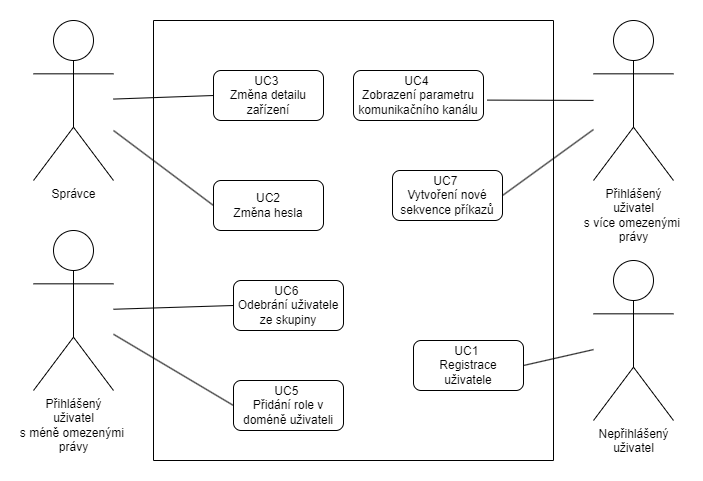
\includegraphics[width=1\textwidth]{images/uc.png}
    \caption{Schéma příkladů použití a jejich očekávaných typických aktérů}
    \label{fig:my_label}
\end{figure}

\def\myprefix{UC}
\begin{enumfunctional}[style=nextline]
\item[Registrace uživatele] 
Nový, zatím nepřihlášený uživatel načte jakoukoliv \acrshort{url} stránku aplikace, díky čemuž bude jako nepřihlášený uživatel přesměrován na přihlašovací stránku. Zde klikne na tlačítko \emph{Register}, které uživatele přesměruje na formulář pro tvorbu nového uživatelského účtu. Po vyplnění potřebných údajů uživatel odešle formulář, server ověří platnost jednotlivých vyplněných formulářových polí, v případě nalezeného problému uživatele nechá údaje ve formuláři upravit a nad formulářem zobrazí notifikaci o neúspěšném vytvoření účtu. V případě úspěchu uživatele automaticky přihlásí a zobrazí notifikaci o úspěšném vytvoření účtu.
\item[Změna hesla]
Uživatel se přihlásí pomocí svých přihlašovacích údajů, které jsou ověřeny. Poté zobrazí detail svého účtu, případně cizího účtu, který chce upravovat, má-li na tuto akci dostatečná práva. Do zobrazeného formuláře pro úpravu uživatelského účtu vyplní nové heslo a formulář odešle. Server validuje pole příchozího formuláře a v závislosti na této validaci heslo změní a zobrazí notifikaci o úspěšné akci, či vrátí předvyplněný formulář k úpravě uživateli a zobrazí notifikaci oznamující neúspěch.
\item[Změna detailu zařízení]
Přihlášený uživatel zobrazí stránku se seznamem všech zařízení, které má právo zobrazit. Z~nich vybere jedno, u kterého bude chtít změnit údaj, například jeho lokaci. V seznamu klikne na identifikační prvek zařízení, jako je jeho jméno, a tím zobrazí detail daného zařízení. Před zobrazením tohoto detailu jsou uživateli zkontrolovány jeho práva, a dle nich se poté detaily zobrazí jako editovatelný nebo needitovatelný formulář. Uživatel změní požadované údaje a klikne na tlačítko \emph{Submit}. Tím je formulář odeslán ke kontrole, a to jak vyplněných údajů, tak opakované kontrole práv odesílajícího uživatele. V závislosti na výsledku těchto kontrol jsou změny popřípadě uloženy. Uživatel je o výsledku informován příslušnou notifikací ve vrchní části obrazovky.
\item[Zobrazení parametru komunikačního kanálu]
Přihlášený uživatel má více způsobů, jak se úspěšně navigovat na stránku zobrazující detail komunikačního kanálu. Pokud kanál není jednoduše identifikovatelný od ostatních kanálů, uživatel nejprve načte stránku seznamu jemu dostupných zařízení. Na ní vybere zařízení obsahující hledaný kanál. Na stránce zobrazující detail zařízení se poté pomocí kliknutí na odkaz v seznamu kanálů daného zařízení dostane na stránku zobrazující detail komunikačního kanálu, na kterém si může uživatel zobrazit všechny parametry.
Pokud ale uživatel zvládne přímo identifikovat hledaný kanál ze seznamu všech kanálů, může využít stránku se seznamem kanálů a díky odkazu ve jméně kanálu přejít na detailní zobrazení komunikačního kanálu v méně krocích. V obou případech však platí, že stránky se uživateli načtou pouze v případě, že má k jejich zobrazení právo. V opačném případě je uživatel přesměrován na domovskou stránku.
\item[Přidání role v doméně uživateli]
Uživatel se přihlásí do aplikace, zobrazí stránku s detailem domény, do které chce roli přidávat. Tuto stránku může najít například pomocí odkazu na stránce obsahující seznam domén. Před načtením tohoto formuláře se však zkontrolují práva uživatele na editaci rolí, a formulář je zobrazen v editovatelném módu pouze v přítomnosti těchto práv. Poté uživatel vyplní přihlašovací jméno účtu, kterému je role přidávána a z menu rolí vybere požadovanou roli. Tento proces může před odesláním formuláře opakovat. Po odeslání formuláře pomocí tlačítka \emph{Submit} jsou hodnoty ve formuláři zkontrolovány vůči předem požadovaným podmínkám, všechny role zmíněné ve formuláři jsou poté zkontrolovány na přítomnost duplikátů, které jsou případně odebrány, a pokud jsou všechny podmínky splněny, nová data jsou uložena do databáze. Zadávající uživatel je o výsledku operace informován notifikací.
\item[Odebrání uživatele ze skupiny]
Přihlášený uživatel zobrazí seznam skupin. V něm vybere skupinu, do které chce přidat uživatele, a zobrazí stránku s jejím detailem pomocí kliknutí na odkaz v názvu skupiny. V tomto detailním zobrazení se uživateli zobrazí mimo jiné tabulka, která obsahuje všechny uživatelské účty, které jsou aktuálně součástí této skupiny. Do tohoto seznamu lze přidat nového uživatele kliknutím na tlačítko \emph{Add} a vyplněním jeho uživatelského jména. Po odeslání formuláře server zkontroluje, zda uživatel s tímto jménem existuje, a při nalezení uživatele a dostatečných právech zadávajícího uživatele je změna uložena do databáze. Zadávající uživatel je poté informován o výsledku operace notifikací.
\item[Vytvoření nové sekvence příkazů]
Přihlášený uživatel zobrazí stránku se seznamem sekvencí. Zde klikne na tlačítko \emph{Add} a tím se přesune na stránku s formulářem, kde může vyplnit detaily nové sekvence. Ve spodní části stránky je dynamicky vytvářená tabulka obsahující jednotlivé kroky sekvence, které mohou být přidávány a odebírány pomocí tlačítka \emph{Add}, resp. \emph{Delete}, které je znázorněno ikonou odpadkového koše. V okamžiku, kdy je uživatel s detaily sekvence spokojen, odešle formulář tlačítkem \emph{Apply}. Server před zapsáním dat do databáze zkontroluje jednotlivé položky a také zkontroluje práva odesílajícího uživatele, pokud jsou v pořádku, operaci umožní. O výsledku je uživatel informován příslušnou notifikací.
\end{enumfunctional}

%---------------------------------------------------------------
\chapter{Návrh}
%---------------------------------------------------------------

\section{Části projektu}
Projekt můžeme rozdělit na serverovou část, běžící u poskytovatele služeb, a klientskou část, jejíž běh zajišťuje na svých lokálních zařízeních uživatel. V následující sekci se budeme zabývat jednotlivými komponentami obou těchto částí, důvody jejich vyčlenění a rozdělení a jejich funkcionalitou.

\subsection{Serverová část}
Serverová část aplikace je bezpochyby komplikovanější a kvůli tomu se skládá z několika komponent. Tou hlavní je \acrshort{nginx} webserver, který pomocí vyhodnocování \acrshort{php} kódu při načtení stránky zajišťuje prezenční a business vrstvu. Dalšími jsou databáze nebo \emph{exekutor}.

Serverovou část tvoří několik vzájemně spolupracujících kontejnerů. Kontejnery se startují buď ze standardních \acrshort{oci} obrazů veřejně dostupných v registru Docker Hub a nebo se startují z obrazů specifických pro tuto práci. Tyto specifické obrazy jsou také veřejně publikovány na Docker Hub a práce obsahuje zdrojové kódy potřebné k jejich vytvoření. 

Kontejnery umožní běh jednotlivých komponent nezávisle na nainstalovaném software a tím odpadají problémy např. s novější (nekompatibilní) verzí knihoven, které se časem mohou objevit. Zároveň je aplikace v kontejneru do značné míry izolovaná a tím celkově zvyšuje bezpečnost ostatních aplikací běžících na tomtéž počítači. Standard \acrshort{oci} zaručí, že je možné kontejnery vytvořit a spustit pomocí různých implementací \enquote{container engine} jako např. Docker, Containerd, CRI-O, Podman, apod.

Aby běh kontejnerů nebyl přerušen výpadky nebo třeba restartem počítače, předpokládám, že bude spouštění a monitorování stavu kontejnerů svěřeno nějakému orchestračnímu nástroji - např. Kubernetes. Já jsem měl pro účely vývoje a demonstrace řešení k dispozici jediný počítač, proto jsem použil jednoduchý orchestrační software Docker Compose.

\subsubsection{Webserver}
Samotný webserver je dvojicí úzce spolupracujících \acrshort{oci} kontejnerů, a to kontejneru \acrshort{nginx} obsahující stejnojmenný software pro zpracovávání příchozích webových požadavků, a kontejneru \acrshort{php}, umožňující interpretaci skriptů napsaných v jazyce \acrshort{php}.

\acrshort{nginx} je první komponentou, která validuje dotazované \acrshort{url}. \acrshort{nginx} řídí své chování mimo jiné podle předpisů popsaných v souboru default.conf. Každé z těchto pravidel má deklarovaný identifikátor a poté akci, která má být provedena. \acrshort{nginx} poté tato pravidla prochází, porovnává jednotlivé identifikátory s dotazovanou \acrshort{url} a snaží se najít co nejkonkrétnější identifikátor. Podle něj poté provede akci.

V našem případě \acrshort{nginx} filtruje od všech dotazovaných \acrshort{url} dotazy na statické zdroje, které se na našem portálu vyskytují ve dvou formách, obrázky a kaskádové styly \acrshort{css}. Každá z těchto forem má vlastní pravidlo. Dotazy na \acrshort{php} generované stránky jsou předávány kontejneru \acrshort{php}, který jazyk \acrshort{php} interpretuje.

\subsubsection{Databáze}
Všechna aplikační data jsem se rozhodl ukládat do databáze. Alternativou by mohly být soubory, ale práce s nimi se v budoucnu hůř škáluje. Jinou alternativou mohou být key-value-store systémy, ale \acrshort{sql} databáze nabízí více možností vyhledávání dat. Rozhodl jsem se využít relační databázi, jelikož data jsou lehce strukturovatelná do tabulek a v těchto tabulkách můžeme jednodušeji využívat kontrolu vstupních datových typů a hodnot. Nyní bylo na místě vybrat jednu z implementací relačních databází. Z mých předchozích osobních zkušeností i recenzí na internetu jsem se rozhodoval především mezi PostgreSQL a MySQL. Obě varianty mají své pro a proti, ve prospěch PostgreSQL hraje například skutečnost, že narozdíl od MySQL umožňuje větší množství specifických výrazů, jako je například \emph{OUTER JOIN} nebo \emph{INTERSECT}, nebo i různé datové typy. PostgreSQL je také rychlejší varianta pro větší a objemnější databáze nebo složitější výrazy. Naše využití ale nepočítá s velkými objemy dat, ani se složitými výrazy, jelikož ve velké míře používáme výrazy pracující pouze s jednou tabulkou a jednou podmínkou. Ačkoliv jsou PostgreSQL i MySQL oblíbenými řešeními s velkými aktivní komunitami a kvalitní dokumentací, z předchozích projektů jsem nabyl pocitu, že hledání řešení pro problémy s MySQL je jednodušší. V závislosti na těchto porovnáních jsem usoudil, že v případě našeho projektu se hodí využít výhod MySQL.

Databáze běží v samostatném kontejneru, který má umožněnou komunikaci s ostatními kontejnery na specifickém portu. Pro jednodušší práci s databází při vývoji nebo údržbě je v projektu přítomen také kontejner Adminer, který umožňuje správu databáze pomocí webového rozhraní. Po přihlášení se administrátorským přístupem lze upravovat schéma databáze i hodnoty v ní uložené, což je důležité pro vývoj a změny
aplikace. V běžném nasazení (v produkci) může být Adminer zcela vynechán.

\subsubsection{Exekutor}

\emph{Exekutor} je jednoduchý Bash skript, který má za úkol eliminovat nevýhodu mého rozhodnutí využít k implementaci hlavní logiky serveru skripty \acrshort{php} spouštěné pouze z požadavků přijatých webserverem. Toto rozhodnutí totiž znamená, že s příchozím požadavkem je spuštěn kód, jehož primárním cílem je generace obsahu vebové stránky, a tento kód je po splnění tohoto cíle ukončen. Server tedy v tuto chvíli nemá možnost cokoliv vykonávat, pokud nepřijde žádný požadavek. Součástí povinností serveru je ale i vykonávání sekvencí, tedy hlídání správného momentu pro vykonání dalšího kroku, a odeslání tohoto kroku zařízení právě ve správný moment, což by bez tohoto skriptu nešlo.

Webserver implementuje specifické \acrshort{url} pro vykonávání časově naplánovaných akcí. Při dotazu \acrshort{http} GET na toto \acrshort{url} webserver provede akce, které v daný okamžik mají být vykonány a odpoví počtem sekund do nejbližší další akce. Skript \emph{exekutor} má jediný úkol, a tím je periodicky načítat tuto stránku, vyjmout z ní údaj o příštím potřebném načtení, počkat na správný moment a poté znovu načíst právě tuto stránku, a tím aktivovat kód serveru. Pro lepší pochopení bychom tedy mohli tento skript popsat jako jakýsi budík, který si sám webserver průběžně nastavuje, a který zajistí, že webserver je ve správný moment probuzen a může tak vykonat svůj úkol.

Tento skript je spouštěn v kontejneru využívající obraz BusyBox, což je obraz který implementuje některé základní prvky linuxového prostředí, díky nimž můžeme skript spustit, ale zároveň nám nepotřebné knihovny a funkcionality nezabírají úložiště ani výkon.

\subsubsection{\acrshort{mqtt} Broker}

\acrshort{mqtt} Broker je kontejner postavený na obrazu Eclipse Mosquitto, který implementuje komunikaci mezi webserverem a jednotlivými komunikačními branami, které slouží k zprostředkování komunikace s jednotlivými \acrshort{iot} zařízeními. Každá z těchto bran se automaticky připojí k tomuto serveru, který se v terminologii \acrshort{mqtt} nazývá Broker neboli zprostředkovatel, a přihlásí se k odběru kanálů příslušících zařízením, která jsou přes danou bránu obsluhována. Tyto fronty pak slouží k předávání informací mezi zařízeními a webserverem a zajišťují, aby se zprávy mezi těmito samostatnými celky úspěšně doručily, i když v moment odesílání zprávy příjemce není dosažitelný. Ve směru ze zařízení k webserveru tato situace nastane, pokud zrovna nebude běžet vyhodnocování stránky \acrshort{php} ať už uživatelem, nebo pomocí automatizovaného \emph{exekutor} skriptu, ve směru z webserveru k zařízení potom takový stav nastává především ve chvíli, kdy je přístup z internetu ke komunikační bráně omezen, a to například nastavením sítě, firewallem, nebo pokud komunikace probíhá přes \acrshort{nat}, jenž zajistí, že komunikace je jednodušeji navazována od klienta směrem k serveru.

\subsection{Klientská část}

Klientská část se skládá pouze z jednoho kontejneru, a tím je kontejner postavený nad obrazem \emph{debian} (s využitím obrazu \emph{gcc}). Tento kontejner spouští kód aplikace komunikační brány, který je napsaný v jazyce C++. Tato aplikace komunikuje se serverem, přesněji řečeno s kontejnerem \acrshort{mqtt} zprostředkovatele, jako \acrshort{mqtt} klient, a jejím úkolem je předávat zprávy z odebíraných témat správným zařízením a naopak. Jelikož chceme zajistit, že tato brána bude umět komunikovat s co největším množstvím jednotlivých zařízení, aplikace podporuje dynamické načítaní knihoven implementujících funkce pro komunikaci mezi bránou a zařízením. Tyto knihovny může vytvořit a přidat k projektu sám uživatel.

%---------------------------------------------------------------
\chapter{Realizace}
%---------------------------------------------------------------

\section{Databázová struktura}

Databáze obsahuje tabulku pro každý ze základních modelů (tedy zařízení, kanál, uživatelský účet, doména, skupina, krok, sekvence, plán sekvence a instance sekvence). Dále v ní najdeme tabulky pro vazby typu N:N (pro vazbu mezi skupinou a zařízením, skupinou a uživatelským účtem, také ale pro přidělení role v doméně konkrétnímu uživatelskému účtu).

\begin{figure}[h!]
    \centering
    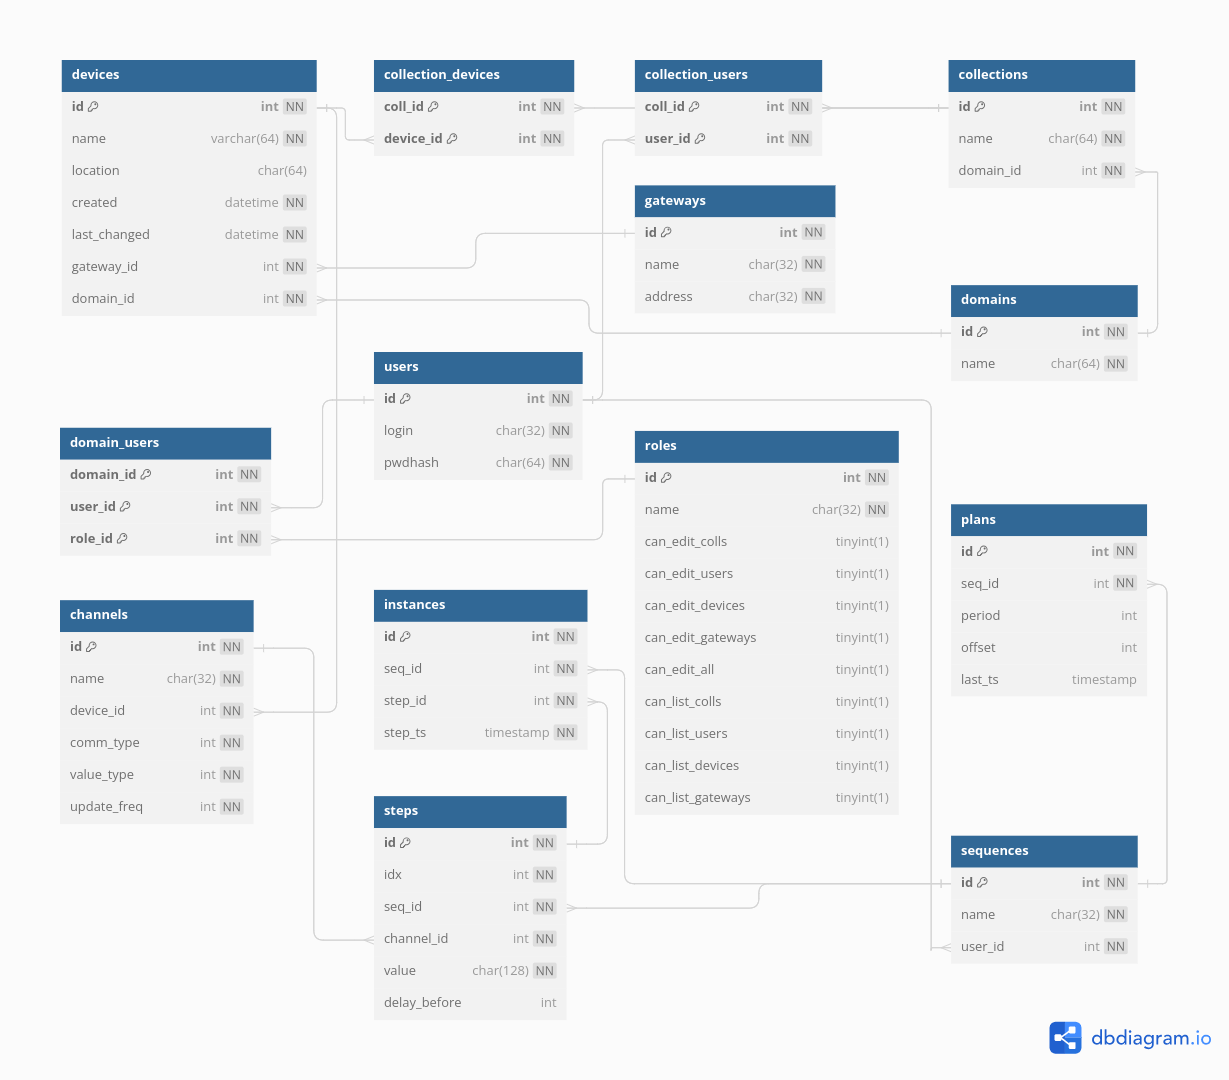
\includegraphics[width=1\textwidth]{images/database.png}
    \caption[Schéma tabulek databáze]{Schéma tabulek databáze \cite[\nopp Figure 1]{database_schema_generator}}
    \label{fig:my_label}
\end{figure}

\subsection{Tabulka zařízení}
Tabulka zařízení \emph{devices} obsahuje kromě sloupce s unikátním identifikátorem \emph{id} sloupce \emph{name} (jméno), \emph{location} (umístění), \emph{created} (datum vytvoření), \emph{last\_changed} (datum poslední změny), \emph{gateway\_id} (ID komunikační brány) a \emph{domain\_id} (ID domény). 

\emph{id} je číselná hodnota unikátní pro každý záznam, která slouží jako primární klíč této tabulky, můžeme tedy podle pouze této hodnoty jednoznačně nalézt hledaný záznam. \emph{location} je uživatelem zvolený popis umístění zařízení; tato hodnota slouží pouze k jednodušší identifikaci zařízení pro uživatele. Náhodným příkladem očekávané hodnoty by bylo například \emph{Obývací pokoj}. 

\emph{created} a \emph{last\_changed} jsou sloupce uchovávající časové hodnoty, v databázi MySQL se typ těchto polí označuje jako DATETIME. \emph{created} je nastavováno přímo databází při ukládání nového záznamu. \emph{last\_changed} by mělo být změněno při každé aktualizaci daného záznamu, sám \acrshort{sql} předpis to však nevyžaduje - režie změny je přenechána na systém, který vytváří \acrshort{sql} výraz pro změnu hodnot v záznamu.

\emph{gateway\_id} je hodnota, která odkazuje na sloupec \emph{id} v tabulce komunikačních bran. Databáze kontroluje existenci záznamu brány s touto hodnotou a neumožní zapsat do tabulky zařízení hodnotu, pro kterou neexistuje záznam v tabulce bran, a zároveň neumožní smazat záznam z tabulky bran, pokud je jeho \emph{id} zmíněno v záznamu v tabulce zařízení. Pro sloupec \emph{domain\_id} platí podobná pravidla, a to tedy že databáze kontroluje existenci záznamu s hodnotou \emph{id} v tabulce domén stejnou jako hodnotou \emph{domain\_id} v tabulce zařízení, a neumožní provést operaci, která by zapříčinila, že pro hodnotu ve sloupci \emph{domain\_id} v tabulce zařízení nebude existovat žádný záznam v tabulce domén, který by totožnou hodnotu měl uloženou ve svém sloupci \emph{id}.

Jelikož se bude tato závislost hodnoty sloupce X v tabulce A na hodnotách sloupce Y v tabulce B objevovat častěji, zadefinujme pojem \emph{sloupec A.X} jako \emph{sloupec X z tabulky A}. Druhým zadefinovaným pojmem nechť je \emph{sloupec A.X odkazuje na B.Y}, znamenající \emph{hodnota v sloupci X.A musí existovat vždy alespoň v jednom záznamu ve sloupci Y.B a tato skutečnost je v každém výrazu upravujícím hodnoty těchto dvou tabulek kontrolována databází}. 

\subsection{Tabulka kanálů}
Tabulka kanálů \emph{channels} je složena ze záznamů pro jednotlivé komunikační kanály všech zařízení. Obsahuje sloupce \emph{id} (unikátní identifikátor), \emph{name} (název), \emph{device\_id} (ID zařízení), \emph{comm\_type} (typ komunikace), \emph{value\_type} (typ hodnoty) a \emph{update\_freq} (frekvence aktualizace).

Sloupec \emph{name} obsahuje krátký název informačního kanálu, například \emph{Vypínání} nebo \emph{Barva}. Hodnota slouží pouze pro lepší identifikaci kanálu pro uživatele. Sloupec \emph{device\_id} odkazuje na \emph{devices.id}, tedy zařízení, jehož kanálem je.

Hodnota \emph{comm\_type} určuje o jaký typ komunikace jde. Databáze podporuje počet typů omezený pouze maximální hodnotou datového typu int, nicméně tato aplikace určuje pouze 3 typy komunikace, a to následující:
\begin{description}
    \item[Jednosměrný kanál od zařízení k serveru,] který bude používán například v kanálu informujícím o aktuální teplotě od teploměru, tedy hodnota, která nemůže být nijak ovládána a je pouze oznamována serveru k zobrazení.
    \item[Jednosměrný kanál od serveru k zařízení,] který bude používán například u aktivace časovaného světla na chodbě, které nepodporuje možnost načtení aktuálního stavu, tedy kanál pro ovládání hodnoty, u které neumíme ověřit její stav.
    \item[Obousměrný kanál,] který bude používán například u zapínání chytrého osvětlení, které umí potvrdit aktuální stav serveru, a ten se tedy může dotázat a na základě výsledku například upravit zobrazení ovládacího prvku tohoto kanálu.
\end{description}
Typ komunikace je v databázi uložen číslem odpovídajícím jeho pozici v seznamu výše.

Sloupec \emph{value\_type} je používán k určení typu hodnot odesílaných v kanálu. Ačkoliv databáze umožňuje větší počet typů, aplikace využívá pouze následující:
\begin{itemize}
    \item{integer}, neboli číselnou hodnotu
    \item{rgb}, neboli trojici číselných hodnot 0-255, představující jednotlivé složky barvy popsané v RGB notaci.
    \item{bool}, neboli binární hodnotu true/false
    \item{string}, neboli posloupnost \acrshort{ascii} znaků v počtu 0-255 znaků.
\end{itemize}
Typ hodnot je v databázi uložen číslem odpovídajícím jeho pozici v seznamu výše.

Sloupec \emph{update\_freq} je délka intervalu, ve kterém se mají hodnoty daného kanálu měnit, v sekundách.

\subsection{Tabulka uživatelských účtů}

Tabulka uživatelských účtů \emph{users} uchovává záznamy, kde každý záznam odpovídá jednomu uživateli. Kromě \emph{id} (jednoznačného identifikátoru) obsahuje také sloupce \emph{login} (uživatelské jméno) a \emph{pwdhash} (výstup hash funkce sha256, jejímž vstupem bylo uživatelem zadané heslo). Sloupec \emph{login} je omezen 32 znaků a databáze automaticky kontroluje, aby hodnoty v něm zapsané byly unikátní. Sloupec \emph{pwdhash} je v databázi deklarovaný jako běžná posloupnost znaků char(64), použití funkce sha256 databáze neprovádí.

\subsection{Tabulka domén}

Tabulka domén \emph{domains} obsahuje údaje o doménách, neboli největších správních celcích v aplikaci. Skládá se ze sloupců \emph{id} (unikátního identifikátoru) a \emph{name} (názvu domény).

\subsection{Tabulka skupin}

Tabulka skupin \emph{collections} zaznamenává jednotlivé skupiny uživatelů a zařízení. Kromě unikátního identifikátoru \emph{id} v ní najdeme také sloupce \emph{name} (jméno skupiny) a \emph{domain\_id} (ID domény). Hodnoty posledního zmíněného sloupce odkazují na sloupec \emph{domains.id}.

\subsection{Tabulka kroků}

Tabulka kroků \emph{steps} ukládá jednotlivé kroky sekvencí a jejich detaily. Používá k tomu sloupce \emph{id} (unikátní identifikátor), \emph{idx} (pořadí kroku v sekvenci), \emph{seq\_id} (ID sekvence), \emph{channel\_id} (ID kanálu), \emph{value} (obsah) a \emph{delay\_before} (pauza před provedením kroku).

Sloupec \emph{idx} obsahuje číslo značící pořadí kroku v sekvenci, které je využíváno pro rychlé hledání následujícího kroku. Sloupec \emph{seq\_id} obsahuje identifikátor sekvence, jejíž součástí je, a jeho data odkazují na sloupec \emph{sequences.id}. Data v sloupci \emph{channel\_id} odkazují na sloupec \emph{channels.id} v záznamu kanálu, ve kterém tento krok komunikuje, sloupec \emph{value} obsahuje data, která budou odeslána v předem zmíněném kanálu. Sloupec \emph{delay\_before} obsahuje čas v sekundách, který my měl být mezi odesláním předchozího kroku, případně spuštěním sekvence, a odesláním tohoto kroku.

\subsection{Tabulka sekvencí}

Tabulka sekvencí \emph{sequences} zaznamenává data týkající se posloupností kroků, které nazývám sekvence, a obsahuje sloupce \emph{id} (unikátní identifikátor), \emph{name} (jméno sekvence) a \emph{user\_id} (ID uživatele, který sekvenci vytvořil). Hodnota sloupce \emph{user\_id} odkazuje na sloupec \emph{users.id}.

\subsection{Tabulka plánů}

Tabulka plánů \emph{plans} je složená ze záznamů, kde každý záznam odpovídá jednomu předem naplánovanému spuštění sekvence. Tento záznam je složený z hodnot \emph{id} (unikátní identifikátor), \emph{seq\_id} (ID plánované sekvence), \emph{period} (četnost spuštění plánu), \emph{offset} (zpoždění spuštění od základní jednotky četnosti) \emph{last\_ts} (časový údaj posledního spuštění plánu). Hodnota \emph{seq\_id} odkazuje na \emph{sequence.id}, 

\subsection{Tabulka instancí}

Tabulka instancí \emph{instances} obsahuje záznamy aktivně běžících sekvencí. Tyto záznam kromě vlastního unikátního identifikátoru \emph{id} uchovává odkaz na sekvenci pomocí sloupce \emph{seq\_id} (ID sekvence), který odkazuje na sloupec \emph{sequences.id}, odkaz na aktuálně plánovaný krok \emph{step\_id} (ID kroku) a časový údaj o čase, ve kterém by měl být tento krok proveden.

\section{Struktura \acrshort{mqtt} komunikace}

Komunikaci pomocí protokolu \acrshort{mqtt} nalezneme v aktuální verzi aplikace mezi \acrshort{mqtt} zprostředkovatelem a webserverem, poté mezi \acrshort{mqtt} zprostředkovatelem a jednotlivými komunikačními branami. Velkým problémem, který nastal v okamžiku rozhodnutí implementovat operační logiku serveru v jazyce \acrshort{php}, navíc způsobem, který nezajišťuje, že bude tato část programu vždy běžící, byla ta skutečnost, že tato část aplikace tak nebude vždy dostupná pro odesílání a především příjem dat. Bylo tedy potřeba zajistit, aby zprávy, které odesílatel serveru odešle právě v momentě, kdy server nebude aktivně vykonávat \acrshort{php} kód a tedy přijímat zprávy, byly serveru uchovány ve frontě, ze které by si je mohl při svém spouštění načíst a tyto zprávy zpracovat.

Způsobů, jak takovou frontu naimplementovat, už je veřejně dostupných hned několik, pro naše účely se jako nejvhodnější volilo použít právě řešení implementující protokol \acrshort{mqtt} \emph{(Message Queuing Telemetry Transport)}. Protokol definuje dva druhy komunikujících stran: zprostředkovatel (\acrshort{mqtt} Broker) a klient (\acrshort{mqtt} Client). \acrshort{mqtt} běží nad protokolem \acrshort{tcp}, kde \acrshort{mqtt} klient je \acrshort{tcp} klientem a navazuje spojení, zatímco \acrshort{mqtt} zprostředkovatel je \acrshort{tcp} serverem a spojení přijímá. Klient odesílá jednotlivé zprávy zprostředkovateli a u každé uvede téma (Topic). Téma slouží jako klíč pro výběr fronty, do které má zprostředkovatel zprávu uložit. \acrshort{mqtt} klient může zprostředkovatele požádat o odběr zpráv pro dané téma.

Témata jsou uspořádána do struktury podobné adresářové cestě v běžných operačních systémech. Techologie \acrshort{mqtt} také podporuje použití zástupných znaků při tvorbě požadavku k odběru. Díky tomu může klient požádat o odběr hned několika souvisejících témat zároveň.

Moje řešení využívá již existující implementaci \acrshort{mqtt} zprostředkovatele \emph{eclipse-mosquitto}, která je dostupná také jako \acrshort{oci} obraz pro použití v kontejneru. Implementace Eclipse Mosquitto umožňuje přidání rozšiřujících modulů, které přidávají nebo upravují funkcionalitu tohoto programu. V projektu jsem se rozhodl využít právě tuto implementaci mimo jiné i právě kvůli jednomu konkrétnímu modulu, kterým je modul \emph{Dynamic Security}. Ten rozšiřuje základní administraci uživatelů / klientů a omezování jejich přístupu k některým tématům, a díky němu lze publikováním konkrétní zprávy ve formátu \acrshort{json} na specifický kanál
upravovat účty, role a jejich přístupy bez nutnosti restartu zprostředkovatele.

Na straně webserveru je použita implementace v jazyce \acrshort{php} s názvem \emph{php-mqtt/client}, dostupná pro instalaci pomocí nástroje Composer z úložiště (repository) Packagist. Pro implementaci \acrshort{mqtt} klienta v jazyce C/C++ jsem se rozhodl využít knihovnu libmosquitto.

\begin{figure}[h!]
    \centering
    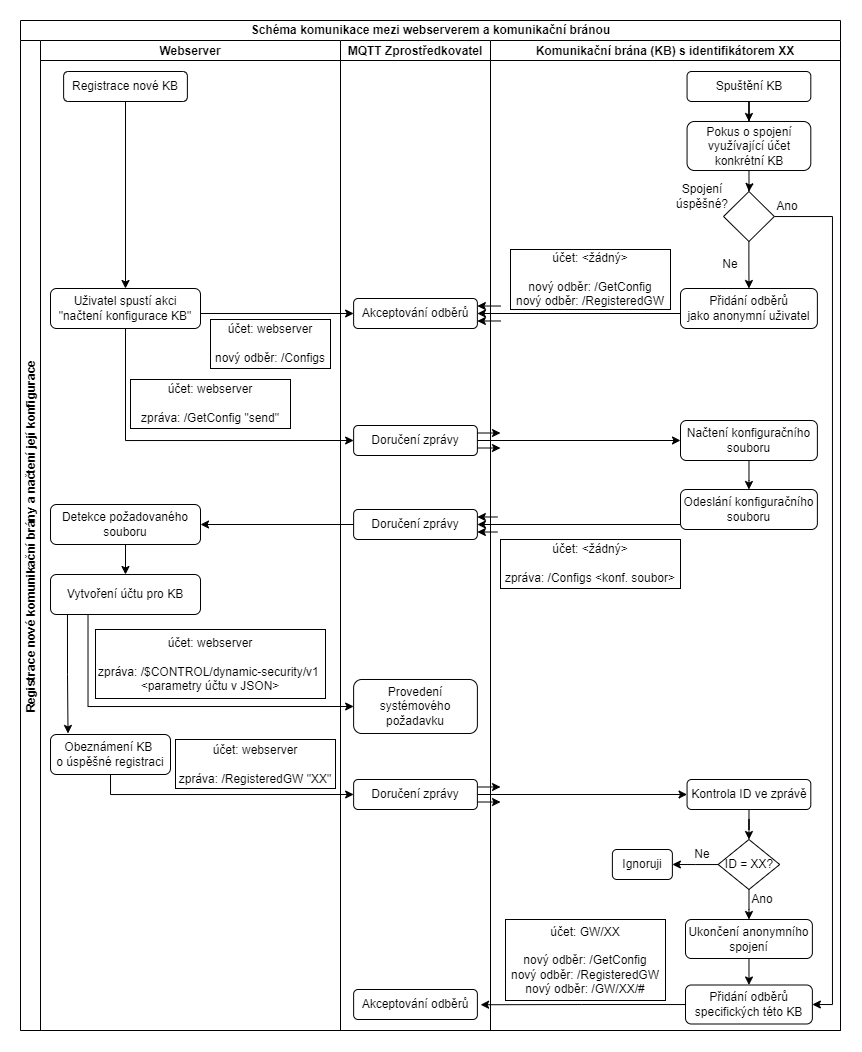
\includegraphics[width=1\textwidth]{images/mqtt-config.png}
    \caption{Schéma procesu registrace komunikační brány a načtení jejího konfiguračního souboru}
    \label{viewClasses}
\end{figure}

\subsection{Přístupové účty}

Cílem tvorby účtů je omezení přístupu jednotlivých \acrshort{mqtt} klientů pouze k tématům, ke kterým by z návrhového hlediska mělo smysl přístup mít. Proto v této aplikaci vytvářím pro každého klienta vlastní účet. V \acrshort{mqtt} zprostředkovateli máme nastavené dva trvalé statické účty a zbytek účtů generujeme dynamicky, jelikož v době tvorby kódu není známé, kolik klientů bude připojeno. 
Statickými účty jsou \emph{administrator} a \emph{webserver}. První zmíněný není používán žádnou komponentou v aplikaci, má absolutní práva a používá se pouze v případě manuálního zásahu administrátorem. Druhý zmíněný je samostatný účet pro webserver, který má statická práva pro odběr na kanály \emph{RegisteredGW} a \emph{Configs} a statická práva pro publikování na kanály \emph{GetConfigs} a \emph{\$CONTROL/dynamic-security/v1}.
Dynamické účty jsou generovány pro každou komunikační bránu, a to s uživatelským jménem dle předpisu \emph{GW/(označení brány)}. Označení brány je v aktuální verzi používaného návrhu komunikace \acrshort{mac} adresa zařízení, na kterém je software komunikační brány spuštěn. Tyto dynamicky vytvořené účty mají poté statická práva pro odběr na kanály \emph{RegisteredGW} a \emph{GetConfigs}, pro publikování na \emph{Configs}. Dále jsou těmto účtům přiděleny dynamická práva na témata vázaná ke konkrétní komunikační bráně.

\subsection{Statická témata}

V této sekci popisuji témata, která se používají po celou dobu běhu programu. Jsou to témata systémová, umožňující měnit nastavení a účty, nebo skupinová, ke kterým má práva k odběru nebo publikování více klientů.

\def\myprefix{}
\begin{enumnonum}[style=nextline]
    \item[GetConfigs]
    Toto téma je využíváno v procesu načítání konfiguračních souborů (dále \acrshort{ks}) z připojených komunikačních bran. Webserver není obeznámen v případě připojení nové brány, proto tedy neposílá žádost o odeslání \acrshort{ks} konkrétně jedné bráně, ale na takzvaný \emph{broadcast topic} - neboli do tématu, ke kterému mají registrovaný odběr všichni uživatelé, nebo alespoň jejich většina. V okamžiku, kdy je do toho tématu publikována jakákoliv zpráva, všechny aktuálně připojené brány publikují svůj \acrshort{ks} do tématu \emph{Configs}. Jelikož potřebujeme, aby nově připojené brány, které dosud neměly vytvořený svůj účet, mohly také publikovat svůj \acrshort{ks} a tak zajistit svou registraci, má právo k odebírání v tomto tématu i anonymní účet.
    \item[Configs]
    Právo k odebírání tohoto tématu má pouze uživatel \emph{webserver}. Funkce tématu \emph{Configs} je sbírat \acrshort{ks} jednotlivých bran a doručit je webserveru, který s nimi může dále pracovat. Je důležité, aby toto téma bylo ochráněno před neautorizovaným přístupem, jelikož právě v této části komunikace jsou přenášeny konfigurační data a osobní údaje. Je to jeden z největších argumentů pro použití modulu \emph{Dynamic Security}, což sice zapříčiní složitější návrh a implementaci, ale zároveň zaručí, narozdíl od varianty, ve které by brány mohly přistupovat k systému pomocí \emph{anonymního účtu}, že si publikované zprávy v tomto tématu nemůže zobrazit žádná třetí strana. Kvůli možné probíhající první registraci nové brány mají k tomuto tématu právo publikovat i brány přistupující pomocí anonymního účtu.
    \item[RegisteredGW]
    Toto téma je používáno k notifikaci brány, že jí byl vytvořen přístupový účet a může tedy začít využívat autentizovaný přístup. Obsahem publikované zprávy je označení brány; stejné, jako brána používá ve svém uživatelském jméně. Právo k odběru tohoto tématu mají jak všechny účty bran, tak i anonymní účet. Pokud brána zachytí svůj identifikátor v publikované zprávě, je to pro ní značení, že má z anonymního přístupu přejít na spojení, ve kterém bude využívat svůj unikátní účet.
    \item[\$CONTROL/dynamic-security/v1]
    Témata s názvem začínajícím znakem \$ jsou dle konvence systémovými, často statistickými či jinak informačními tématy. Lze je přirovnat k primitivnímu konzolovému přístupu, kdy publikováním perfektně formulovaných zpráv lze docílit změn v nastavení. Na některá témata pro změnu publikuje přímo \acrshort{mqtt} broker, lze z nich vyčíst záznamy událostí, jako lze u jiných platforem z \emph{log} souborů.
\end{enumnonum}

\subsection{Dynamicky vytvářená témata}

Pro doručování běžných zpráv jako je informace o aktuálním stavu komunikačního kanálu zařízení nebo odeslání nové hodnoty v tomto kanálu se využívají dynamicky generovaná témata pro každé zařízení a jeho kanály. Názvy témat mají tvar \emph{GW/(identifikátor brány)/(identifikátor zařízení)/(identifikátor kanálu)}. Identifikátorem zařízení i kanálu jsou v tomto kontextu jejich jména. Ačkoliv by se totiž na první pohled mohlo zdát, že je mnohem lepší i identifikaci využít pro tento účel vytvořené hodnoty sloupců \emph{id} v tabulce \emph{devices}, respektive \emph{channels}, tyto hodnoty zná pouze webserver, komunikační brána by podle nich tedy nebyla schopná identifikovat adresáta.

\section{Serverová část aplikace}

V této části práce rozeberu detailně implementaci požadavků na straně serveru. Budu rozebírat jednotlivé části kódu aplikace a popisovat, proč jsem se rozhodl k právě tomuto řešení. Serverová část aplikace je zdaleka nejobsáhlejší částí práce, alespoň co se objemu kódu týče. Seznam níže popisuje adresářovou strukturu a zmiňuje významné soubory a jejich lokaci.

\begin{figure}[h!]
    \dirtree{%
		.1 conf.
            .2 default.conf\DTcomment{konfigurační soubor programu \acrshort{nginx}}.
            .1 html\DTcomment{adresář statických zdrojů webových stránek}.
            .2 css\DTcomment{adresář \acrshort{css} souborů pro webové stránky}.
            .2 icon\DTcomment{adresář obrázků a ikon}.
            .1 mqtt\DTcomment{adresář využívaný \acrshort{mqtt} zprostředkovatelem}.
            .2 config.
            .3 mosquitto.conf\DTcomment{konfigurační soubor \acrshort{mqtt} zprostředkovatele}.
            .3 mqttpass\DTcomment{soubor uchovávající \acrshort{mqtt} účty}.
            .2 dynamic-secutiry.json\DTcomment{konfigurační soubor modulu \emph{Dynamic Security}}.
            .1 php\DTcomment{adresář zdrojových kódů webových stránek}.
            .2 app\DTcomment{adresář zdrojových kódů specifických projektu}.
            .3 model\DTcomment{adresář kódů modelových tříd}.
            .3 view\DTcomment{adresář kódů zobrazovacích modulů stránky}.
            .2 framework\DTcomment{adresář obecných zdrojových kódů}.
            .3 controller\DTcomment{adresář kódů ovladačů modelů}.
            .3 model\DTcomment{adresář kódů modelových tříd}.
            .3 view\DTcomment{adresář kódů zobrazovacích modulů stránky}.
            .1 php-image\DTcomment{adresář pro tvorbu \acrshort{oci} obrazu dandadin/iothome-php}.
            .1 docker-compose.yml\DTcomment{konfigurační soubor programu Docker Compose}.
            .1 executor\DTcomment{skript modulu \emph{Exekutor}}.
	}
    \caption{Graf adresářové struktury serverové části aplikace}
    \label{fig:my_label}
\end{figure}



\subsection{Webserver}

Jak bylo v návrhové části práce zmíněno, webserver je složen ze dvou spolupracujících částí; programu, který zajišťuje komunikaci pomocí protokolů \acrshort{http} nebo \acrshort{https} s klientem a doručení správného obsahu klientovi jako odpověď na jeho dotaz, a \acrshort{php} interpreta, tedy programu, který rozumí kódu v jazyce \acrshort{php}, provede skript, který byl požadován, a výsledek předá k odeslání klientovi.

\subsubsection{Volba použitých technologií}

K implementaci první, komunikační části, se v běžných projektech vyskytuje téměř vždy jedno ze dvou konkrétních řešení, a těmi jsou \acrshort{nginx} a Apache. Obě řešení jsou ve většině parametrů srovnatelné, zaměnitelné, a z osobní zkušenosti bych si odvážil tvrdit, že největším faktorem při výběru mezi těmito řešeními bude nejspíše pro většinu uživatelů jejich osobní preference nebo zkušenost. Pokud bych měl pojmenovat alespoň pár rozdílů mezi nimi, zmínil bych, že Apache vytváří nové vlákno pro každé příchozí spojení, zatímco \acrshort{nginx} zvládne obsluhovat několik připojení najednou, což může zajišťovat mírné zlepšení výkonnosti \acrshort{nginx}. \acrshort{nginx} zvládá rychleji načítání statického obsahu, bohužel ale často pro dynamický obsah, jakým je právě například \acrshort{php} stránka, vyžaduje instalaci přídavných modulů nebo programů, zatímco Apache často dynamický obsah zvládne zpracovat sám. Nejen díky předchozím osobním zkušenostem jsem se tedy rozhodl využít řešení \acrshort{nginx} a k němu přidat interpreta pro jazyk \acrshort{php}.

Všeobecně doporučovaným rozšířením je program \acrshort{php-fpm}. Jak \acrshort{nginx} tak \acrshort{php-fpm} jsou dostupné ve vlastním \acrshort{oci} obrazu, dle kterého jsem vytvořil spolu komunikující Docker kontejnery. K jejich propojení stačí jen zajistit, aby bylo v konfiguračním souboru \acrshort{nginx} vytvořeno pravidlo pro dotazy na \acrshort{php} stránky, které odkáže na program \acrshort{php-fpm}.

V projektu ale využívám i veřejně dostupné knihovny, na kterých závisí vyhodnocování mnoha částí \acrshort{php} kódu. Pro jejich snadnou instalaci, správu a uchovávání lze využít programu Composer. Pokud tvůrce nahraje svou knihovnu v předem daném formátu do jednoho z mnoha repozitářů, tedy serverů pro úschovu balíčků, jakým je například Packagist, uživateli, který ho chce využít ve svém projektu pak stačí zahrnout jeho jméno a požadovanou verzi do konfiguračního souboru programu Composer, který balíček stáhne, připraví a dokonce v případě potřeby stáhne i další balíčky, na kterých je daný balíček závislý. Všechny stažené balíčky jsou pak uloženy do souboru \emph{composer.lock}, který uchovává jeho kompletní aktuální verzi, díky čemuž se nemusíme obávat problému, který by mohl nastat, kdyby byl balíček z portálu stažen. Zároveň je však pomocí tohoto programu jednoduché verzi balíčku změnit nebo nainstalovat jiný, a to bez ruční manipulace se soubory.

Composer lze nainstalovat dle oficiálního návodu i do Docker kontejneru, a to pomocí technologie \emph{multi-stage build}. Docker poté při procesu výstavby kontejneru postupuje dle předem vytvořeného postupu, který může obsahovat několik příkazů které mohou výstavbu ovlivnit. Nabízí také možnost provést výstavbu jiného kontejneru, která je dokončena v průběhu původní výstavby, a lze tak využít libovolnou část pomocného kontejneru k výstavbě požadovaného celku. V našem projektu je tato technologie konkrétně využita tak, že při výstavbě kontejneru \acrshort{php-fpm} je vytvořen kontejner Composer, ze kterého je využit a překopírován spustitelný soubor samotné aplikace Composer do právě vytvářeného kontejneru. Dále pak využijeme přímo při výstavbě aplikaci Composer, které oznámíme potřebné knihovny a ty jsou tak nainstalovány ještě před prvním spuštěním.

Při rozhodování mezi veřejně dostupnými knihovnami implementujícími \acrshort{mqtt} klienta pro \acrshort{php} s bezplatnou a adekvátní licencí jsem neměl na první pohled očividného favorita, nakonec jsem se ale dle uživatelských recenzí, množství dostupné dokumentace a předpokládané obtížnosti implementace rozhodl využít balíček \emph{php-mqtt/client} dostupný na portálu Packagist. Toto rozhodnutí se ale v průběhu implementace ukázalo jako poměrně nešťastné, jelikož jsem v implementaci komunikace s \acrshort{mqtt} zprostředkovatelem nalezl chybu přímo v této knihovně. Díky dostupnosti zdrojových kódů knihovny se mi povedlo problém lokalizovat a dokonce i upravením kódu knihovny opravit, nicméně tato úprava byla provedena pouze na mé lokální kopii a nebyla veřejně dostupná. Proto jsem do výstavby \acrshort{php-fpm} kontejneru přidal ještě soubor formátu \emph{patch}, který provedené změny popisuje stylem příkazu \emph{diff}, a pomocí příkazu \emph{patch} potom tyto změny promítám do adekvátních souborů. Poté už stačí při výstavbě kontejneru nainstalovat rozšíření pro komunikaci s MySQL databází a kontejner je připraven.

Jelikož je tento proces výstavby poměrně složitý, závislý na dostupnosti obrazu \acrshort{php-fpm}, obrazu Composer, ale i rozšíření pdo-mysql, a musel by ho provádět každý uživatel při počáteční instalaci webserveru, rozhodl jsem se vystavěný obraz nahrát na registr Docker Hub. Ten zajišťuje, že veškeré obrazy použité při výstavbě a v té době dostupné na Docker Hub zůstanou dostupné doživotně. Zároveň byla na DockerHub nahrána i data nainstalované verze pdo-mysql, díky čemu byly všechny tyto závislosti odstraněny. Nahrání nové verze balíčku na DockerHub je prováděno automaticky pomocí technologie GitHub Pipelines, použité v GitHub úložišti tohoto projektu. Při provádění akce \emph{git push} do úložiště GitHub ověří, zda nedošlo ke změně souboru \emph{php-image/tag}, ve kterém je uložena značka verze, pro kterou je předpis pro výstavbu připraven. Pokud je změna detekována, jednoduchý skript nový předpis sám nahraje na registr DockerHub, kde je poté připraven ke stažení.

\subsubsection{Exekutor}

\emph{Exekutor} je část projektu, která zajišťuje, že webserver nebude trpět jednou z největších nevýhod řešení, jehož běh je vázaný na \acrshort{http} dotazy jeho uživatelů. Bez této části projektu by webserver umožňoval bez problémů obsluhovat veškeré dotazy a průběhu jejich vyhodnocování komunikovat s databází, dynamicky generovat obsahy stránek a obecně splňovat téměř všechny své povinnosti, nicméně problém nastane u činností, které musí být provedeny v přesný, předem určený čas. Pokud by webserver na tento čas čekal způsobem, kdy by po přijetí spojení nepřetržitě běžel a čekal tak až na moment, kdy má vykonat požadovanou instrukci, narazil by na možný fatální problém, a tím je ukončení spojení, které by ukončilo jeho vykonávání. Běžné spojení pomocí \acrshort{http} má totiž nastavený timeout neboli časovač, a pokud do vypršení tohoto časovače klient nedostane od serveru odpověď, spojení ukončí. Tento časovač bude u většiny prohlížečů v řádu desítek sekund, maximálně minut, webserver by ale následující instrukci mohl mít naplánovanou ale až na týden dopředu.

Pokud by se ale webserver spoléhal pouze na náhodná spojení od uživatelů, která budou v závislosti na fázi dne přicházet nerovnoměrně, a vykonával časované úkony pouze když přijme dotaz na jakoukoliv stránku, pravděpodobně by tyto úkony nebyly provedeny včas. Ideálním řešením by bylo, pokud by oddaný uživatel odeslal požadavek maximálně pár sekund před tím než nastane moment provedení úkonu. Jelikož se na existenci takového uživatele nemůžeme spolehnout, jeho funkci přebírá právě \emph{exekutor}, jehož jediným úkolem je zjistit, kdy má být webserver aktivován a ve správný čas odeslat požadavek.

Aby byla zachována jednoduchost implementace na straně \emph{exekutoru}, který je psán jako Bash skript, zvolil jsem jako způsob jednosměrné komunikace mezi webserverem a tímto skriptem obsah stránky, který je vygenerován webserverem a načten jako klasické čtení souboru skriptem. Při přijmutí dotazu na tuto \acrshort{url} server z databáze všech plánovaných kroků vybere ten záznam, který má čas plánovaného provedení nejdříve, vypočte, kolik sekund zbývá do toho momentu, a tento počet vypíše jako jediný obsah na stránce. \emph{Exekutor} tento počet sekund čeká a poté znovu načte tuto stránku, čímž aktivuje webserver právě v požadovanou chvíli. Problém by však nastal, pokud by v čase, kdy \emph{exekutor} čeká na vypršení požadovaného času, webserveru přibyl nový plánovaný krok, který by měl být zpracován dříve. Proto \emph{exekutor} čeká na příchozí \acrshort{udp} spojení na předem definovaném portu, a v okamžiku, kdy toto spojení přijde, \emph{exekutor} přeruší čekání na fixní dobu a okamžitě se spojí s webserverem pomocí načtení výše zmíněné \acrshort{url} a tím ho okamžitě aktivuje a zároveň aktualizuje informaci o čase, který má čekat. \acrshort{udp} spojení je sice jednodušší na implementaci než spojení \acrshort{tcp}, nicméně má vůči němu také jisté nevýhody a jednou z nich je skutečnost, že datagram \acrshort{udp} nemusí být doručen a odesílatel to nemusí zjistit. Vzhledem k tomu, že exekutor a webserver ve většině skutečných implementací poběží na stejném počítači, ke ztrátě \acrshort{udp} datagramů prakticky nedochází. Ikdyby přesto ke ztrátě \acrshort{udp} došlo, dojde ke zdržení naplánované akce maximálně o dobu, po kterou exekutor čeká. Proto je v současné aplikaci omezena doba čekání exekutora na maximálních 30 sekund. Sám webserver tedy po nalezení nejčasnějšího plánovaného kroku porovná počet sekund do tohoto momentu s fixní hodnotou 30 sekund a menší hodnotu z těchto dvou předá v odpovědi \emph{exekutoru}. To zajistí, že i v případě nedoručeného \acrshort{udp} datagramu, informujícího \emph{exekutora} o nutnosti opětovného načtení informací z webserveru kvůli novému naplánovanému kroku s dřívějším datem provedení bude průměrné zdržení 15 sekund, což je u předem plánovaných kroků akceptovatelné zdržení. Pokud by uživatel potřeboval jistotu provedení v dřívějším čase, nemusí využívat funkcionalitu plánovaných kroků a manuálně obsah kroku spustit sám.

\begin{figure}[h!]
    \centering
    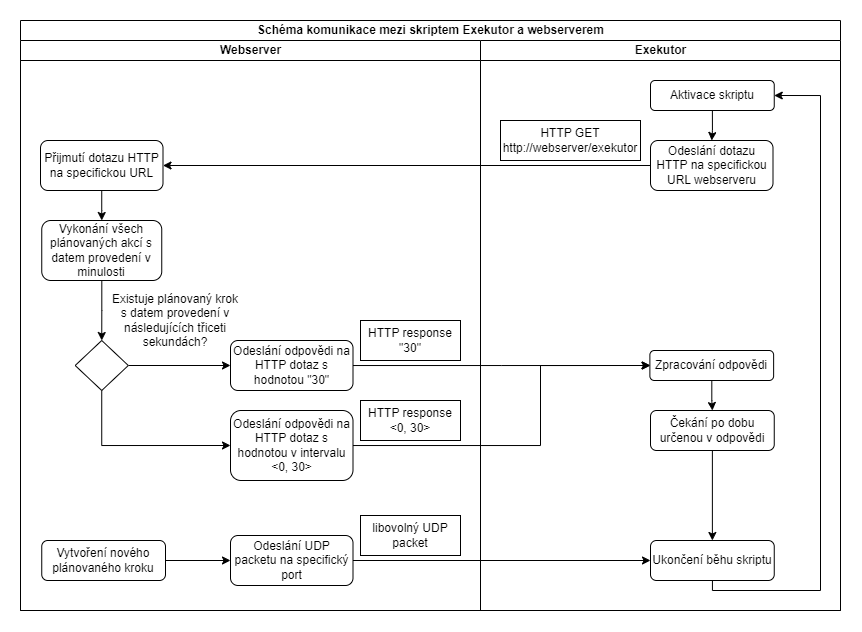
\includegraphics[width=1\textwidth]{images/exekutor.png}
    \caption{Schéma funkcionality modelu \emph{Exekutor} a jeho komunikace s webserverem}
    \label{viewClasses}
\end{figure}

\subsubsection{Architektura tříd programu}

Uživatelské rozhraní jsem implementoval podle návrhového vzoru Model-View-Controller (\acrshort{mvc}). Projekt je tvořen množstvím spolupracujících tříd, které bychom mohli až na výjimky rozdělit do třech částí, a těmi jsou \emph{View}, \emph{Model} a \emph{Controller} (neboli \emph{Pohled}, \emph{Model} a \emph{Ovladač}).

\paragraph{View} \hfill

\begin{figure}[h!]
    \centering
    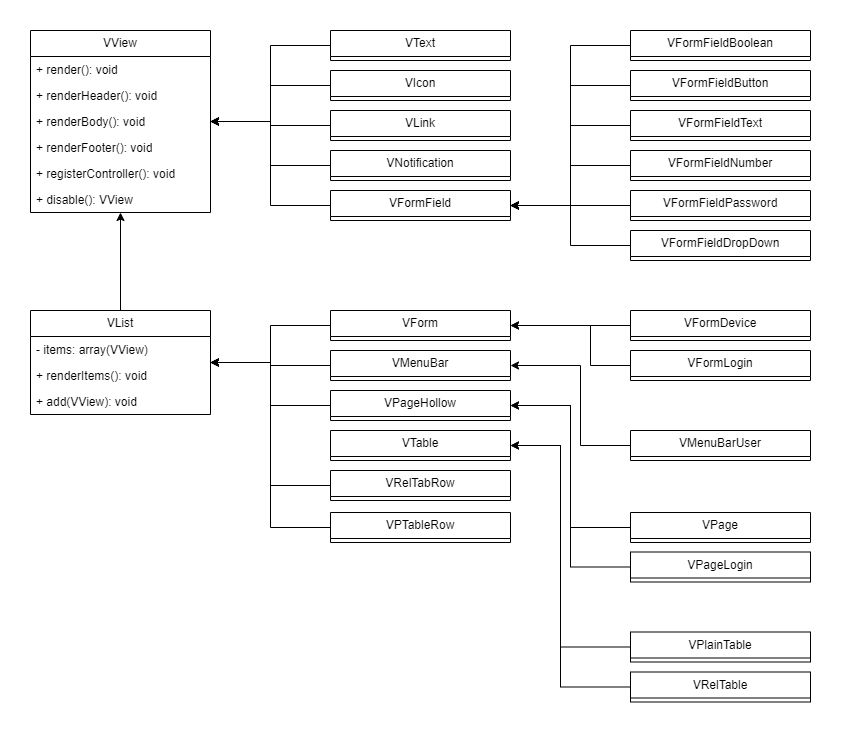
\includegraphics[width=1\textwidth]{images/view-tridy.png}
    \caption{Schéma dědičnosti vybraných tříd typu \emph{pohled}}
    \label{viewClasses}
\end{figure}

Třídy typu \emph{View}, neboli \emph{Pohled}, jsou třídy, které zajišťují vygenerování zobrazitelného \acrshort{html} kódu. \acrshort{html} kód generují na základě dat získaných z databáze a aktuálním stavu editovaného objektu, který je uložen v příslušné třídě Model. Pohledy mohou být i kontejnerem, který ve svém zobrazování využívá jiné pohledy. V takovém případě si uchovává seznam pohledů, které ke svému zobrazení vyžaduje, a případnou aktivaci jeho metod poté propaguje i do těchto pohledů. 

Třídy typu \emph{Pohled} mají na začátku svého jména \emph{V} pro jednodušší odlišení. Jejich společným předkem je třída \emph{VView}, která je abstraktním pohledem a deklaruje metody \emph{render}, dále využívající metody \emph{renderHeader}, \emph{renderFooter} a \emph{renderBody}, \emph{disable} a \emph{registerController}. Metody obsahující ve svém názvu slovo \emph{render} jsou využívány pro generování výsledného \acrshort{html} obsahu stránky, přičemž odvozené třídy mohou tyto metody předefinovat a generovat vlastní specifický obsah. Ačkoliv přesné využití těchto metod zůstává na vývojáři aplikace, myšlenka za návrhem byla taková, že pokud odpovídá daný pohled jedné \acrshort{html} značce, pomocí metody \emph{renderHeader} by měla být vytvořena jeho otevírací verze, pomocí \emph{renderFooter} jeho uzavírací verze a pomocí \emph{renderBody} celý obsah, který by měl být mezi nimi. Metoda \emph{disable} je využívána pouze některými pohledovými třídami, a to především třídami implementující formulářová pole. Pomocí této metody totiž můžeme dogenerovat kód potřebný k zajištění, že uživatel, zobrazující tento pohled, nebude moci data v něm obsažená nijak změnit. Metoda \emph{registerController} je pak využívána u pohledových tříd, které vyžadují použití ovladače, a v této metodě mohou svůj ovladač zaregistrovat, tedy ho aktivovat a připravit pro načítání příchozích dat. 

\paragraph{Model} \hfill

\begin{figure}[h!]
    \centering
    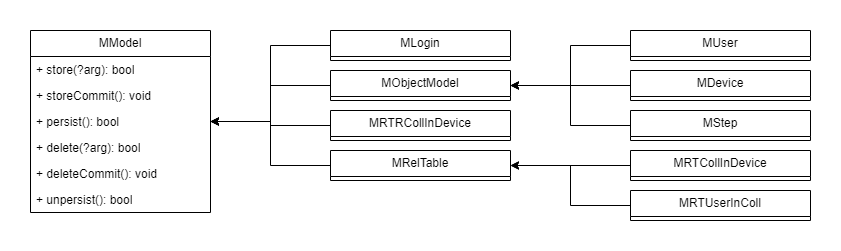
\includegraphics[width=1\textwidth]{images/model-tridy.png}
    \caption{Schéma dědičnosti vybraných tříd typu \emph{model}}
    \label{viewClasses}
\end{figure}

Modelové třídy reprezentují právě editované objekty (datové struktury) podobné těm, které jsou ukládány do databáze. Udržují stav editovaného objektu mezi jednotlivými odesláními \acrshort{html} formuláře a tento stav pak na závěr zapíší do databáze, pokud uživatel klikne na tlačítko uložit. Každý z modelů obsahuje proměnné, které z většiny odpovídají jednotlivým sloupcům adekvátní databázové tabulky, nicméně v případě některých objektů, například těch, které mezi sebou mají M:N vazbu, se mohou tyto proměnné mírně odlišovat. Jelikož ve většině případů chceme mít možnost editovat M:N vazby spolu s editací jednoho z objektů v této vazbě, například na webovém portálu uchovávajícím recepty a ingredience do nich použité, preferujeme možnost upravovat využité ingredience přímo ve stejném formuláři, jako editujeme jiné vlastnosti receptu, třeba jeho název, potřebujeme do některých modelů přidat ještě informace z jiných tabulek. O tento proces se stará právě konstruktor modelové třídy, která dále obsahuje metody \emph{store}, \emph{storeCommit}, \emph{persist}, \emph{delete}, \emph{deleteCommit} a \emph{unpersist}, které jsou definované společným předkem, třídou MModel.

První tři zmíněné metody jsou používány k ukládání aktuálního modelu do databáze, poslední tři poté o odebrání adekvátních dat z databáze.
Ukládání dat je implementované pomocí databázových transakcí. Pokud bych měl databázové transakce popsat člověku, který o nich zatím neslyšel, řekl bych mu, že transakce je seznam operací, před jejichž provedením je stav databáze uložen, a po dokončení těchto operací se může uživatel rozhodnout, zda je s výsledkem spokojený a transakci potvrdí, čímž je starý stav databáze přepsán nově vytvořeným, nebo zda transakci zruší, kdy je nový stav zapomenut a používá se verze vytvořená před začátkem transakce. Tuto logiku implementuje metoda \emph{persist}, která započne transakci, provede metodu \emph{store}, která provádí samotné operace ukládání dat, a pokud se tato metoda ukončí s pozitivní návratovou hodnotou, potvrdí aplikování transakce databázi, a aktivuje metodu \emph{storeCommit}, ve které model implementuje činnosti, které je potřeba provést pouze v případě úspěšného uložení. V opačném případě transakci zruší. Na velmi podobném principu operují i metody pro mazání dat z databáze, kdy metoda \emph{unpersist} spravuje transakci obdobně jako metoda \emph{persist}, \emph{delete} implementuje samotné mazání dat a \emph{deleteCommit} je aktivována pouze po úspěšném dokončení transakce.

\paragraph{Controller} \hfill

\begin{figure}[h!]
    \centering
    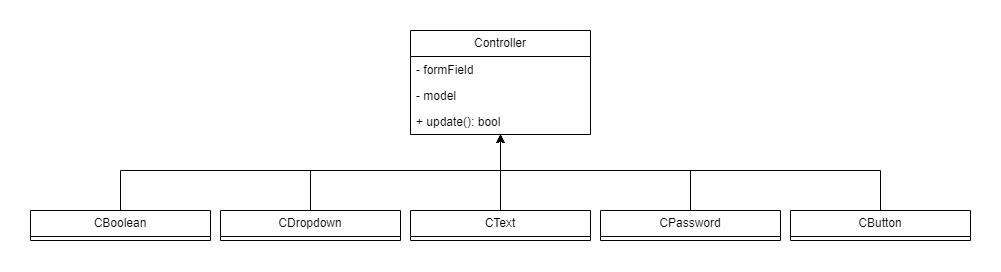
\includegraphics[width=1\textwidth]{images/controller-tridy.png}
    \caption{Schéma dědičnosti vybraných tříd typu \emph{ovladač}}
    \label{viewClasses}
\end{figure}

Třídy typu \emph{Controller} (\emph{Ovladač}) slouží k automatickému předání příchozích dat obsažených v \acrshort{http} požadavku příslušným modelovým objektům. Objekty jsou totiž mezi jednotlivými dotazy v jedné relaci za určitých podmínek uchovány a je potřeba v nich změnit některé proměnné dle aktuálních přijatých dat, aby poté mohly být uloženy do databáze. Data na stránce však nejsou jednoduše napárovatelná na jednotlivé proměnné v modelu, takže je potřeba naimplementovat systém, pomocí kterého bude jednoznačně dáno, která příchozí informace má být uložena do konkrétní proměnné v určitém modelu. Dále je také u některých dat potřeba provést jejich validaci nebo transformaci, jedním z příkladů může být například obsah jakéhokoliv formulářového pole typu \emph{password} neboli \emph{heslo}, u kterých chceme, aby byl jejich obsah uložený na co nejméně místech. Při tvorbě určitého \emph{pohledu} už víme, že jde o část stránky, která má mít možnost doručit informaci od uživatele k serveru, jako je například kliknutí na tlačítko, nebo vyplnění pole ve formuláři. Proto je už tedy při generaci stránky jako následující krok po vytvoření všech \emph{pohledů} zavolána na kořenový \emph{pohled} metoda \emph{registerController}, která je dále propagována na všechny zanořené \emph{pohledy}. Jako parametr této metody je objekt typu \emph{FormContext}, který se chová jako chytrý seznam dvojic určitého \emph{ovladače} a k němu spárované proměnné z modelu. \emph{FormContext} je poté uložen jako součást pole \emph{\$\_SESSION}, které je unikátní pro jednotlivou \acrshort{http} relaci a server ho uchovává mezi jednotlivými dotazy. Po přijmutí dat od uživatele je poté \emph{FormContext} načten z tohoto pole a pomocí jeho metody \emph{updateModel} jsou nalezeny všechny \emph{ovladače}, pro které mohly být přijaty nová data, a ty pomocí metody \emph{update} tyto data načtou z pole \emph{\$\_POST}, zpracují a transformují hodnoty a uloží je do příslušného modelu. Tento proces aktualizace modelů probíhá ještě před započetím vytváření \emph{pohledů} použitých uvnitř stránky, která bude uživateli odeslána jako odpověď na jeho \acrshort{http} POST dotaz.

\subsubsection{Handler}

Celý proces zpracování požadavku začíná převzetím přijatého požadavku z kontejneru \acrshort{nginx}, které probíhá kódem v souboru \emph{handler.php}. Tuto část nazývám \emph{Handler}. Ten má za úkol rozhodnout, zda je požadavek platný, tedy zda splňuje náležitosti, které od něj očekáváme, jako je například zda se dotazuje na existující stránku, a zda jde o běžný požadavek, který je dále vyhodnocován soustavou tříd, nebo jde o požadavek servisní, jakým je například spojení navázané z modulu \emph{Exekutor}, tedy požadavek, který byl vytvořen jinou částí aplikace a nepochází od uživatele. Pod požadavkem, který by byl v tuto chvíli označen jako neplatný, si můžeme představit například požadavek na neexistující \acrshort{url}, nebo požadavek, který neobsahuje vyžadovaná potřebná data v hlavičce.

V případě běžného platného požadavku \emph{Handler} dle dotazované \acrshort{url} rozhodne, jaká stránka byla uživatelem vyžadována, a vyhledá název třídy, která je jejím \emph{pohledem}. Každý pohled, který může být v této situaci vyžadován, má implementovanou statickou metodu \emph{checkPermissions}, jejíž parametrem můžeme dále specifikovat daný požadavek, a to například zda bylo v požadované \acrshort{url} přítomné \emph{id} objektu, jehož zobrazení či editaci chceme provést, nebo zda se jedná o požadavek o vytvoření nového záznamu pro jednu z entit jako zařízení nebo uživatelský účet. Tato metoda ověří, zda aktuálně přihlášený uživatel má právo na přístup k požadované stránce.

V případě nedostačujících práv je poté odeslána \acrshort{http} odpověď pomocí funkce \emph{header(\enquote{Location: }.\$newUrl)}, která uživatele přesměruje na \acrshort{url} popsanou v proměnné \emph{newUrl}, která je ve většině případů nastavena na kořenovou stránku aplikace. Pro uživatele to tak znamená, že i případě pokusu o načtení stránky, ke které nemá právo přístupu, je mu zobrazen určitý obsah; z kořenové stránky se také může jednoduše navigovat na stránky, které mu mohou být zobrazeny. Pokud má uživatel dostatečná práva, je vytvořena instance hlavního kořenového \emph{pohledu}, která ve svém konstruktoru vytvoří instance všech potřebných atomických \emph{pohledů}, které budou na celé stránce použity. V okamžiku dokončení tohoto konstruktoru už je celá struktura stránky vytvořena v paměti serveru, nicméně stále není součástí odpovědi klientovi. Tou se stane až po dokončení metody \emph{render}, která je jako další krok zavolána u instance kořenového \emph{pohledu} stránky. Tato metoda se také propaguje do všech závislých \emph{pohledů} a každý z nich připojí ve správném pořadí do výstupu \acrshort{php} kódu část \acrshort{html} odpovídající té části stránky, kterou představuje právě daný \emph{pohled}. 



\subsection{Komunikační brána}

V této sekci je popsána část softwaru označována \emph{komunikační brána}. Ta slouží k zajištění komunikace mezi jednotlivými zařízeními a aplikační serverovou strukturou. 

V ideálním případě by komunikace mezi zařízením a serverem mohla být navázána oboustranně nezávisle na okolních faktorech. V reálných případech využití ale zařízení, se kterými server komunikuje, mohou být nejen geograficky rozmístěny po celé planetě, ale často také připojeny z určité místní sítě, kterou může být jak podniková síť sloužící pro připojení všech zařízení na pobočce, tak i klasická síť domácí. Tyto sítě jsou pro jednodušší správu a především zvýšenou bezpečnost odděleny od přímého přístupu do zbytku Internetu jako takového zařízením jako je například router, který implementuje předem nastavená síťová pravidla jako je \acrshort{nat} nebo firewall, aby zabránil potenciálně nebezpečným spojením. Pro výše zmíněnou komunikaci to znamená, že bez předchozího nastavování těchto pravidel nelze provést připojení ze strany serveru směrem k zařízení, jelikož v případě existujících pravidel firewall bude naše spojení pravděpodobně nečekané a tedy zablokované, v případě \acrshort{nat} vzniká problém, že IP adresa zařízení na vnitřní síti není dostupná (routable) z vnější sítě. Data mohou být doručena pouze na hranici této sítě, ale server se nemůže spolehnout, že zařízení, které na hranicí sítí tento požadavek přijme, bude schopné rozhodnout, kterému zařízení zprávu předat, a ta tak pravděpodobně nebude doručena. 

Takový problém je v praxi řešen dvěma způsoby, a to tak, že jsou buď všechna tato pravidla upravena, aby bylo spojení proveditelné, ale zároveň zůstaly v co největší míře zachovány kladné vlastnosti těchto pravidel, nebo dvě zařízení, které vyžadují možnost komunikovat mezi sebou, využijí návrhového vzoru, ve kterém bude spojení navazovat strana \emph{klienta} (v tomto případě komunikační brána), a to i v případě, že data mají téci v opačném směru. Pokud bude strana komunikační brány udržovat spojení neustále otevřené, nebo ho bude alespoň obnovovat po dostatečně malé odmlce, zdržení zprávy mířící ze serveru k bráně v době, kdy spojení zatím nebude navázané, nebude významné.

Komunikace mezi serverem a komunikační branou probíhá pomocí protokolu \acrshort{mqtt}. Tato skutečnost zjednodušuje implementaci na straně serveru, jelikož integrace potřebných knihoven pro implementaci protokolu \acrshort{mqtt} už server obsahuje. \acrshort{kb} využívá knihovnu \emph{libmosquitto}.

\subsubsection{Implementace}

Software \emph{komunikační brány} je psán v jazyce C++, jelikož je to dle mého názoru jazyk, který je všeobecně velmi rozšířený a drtivá většina vývojářů se s ním při vývoji aplikace setkala, což je důležité, jelikož předpokládám, že si mnoho vývojářů využívajících tento software budou vytvářet vlastní komunikační moduly. Výhodou je také relativní nenáročnost na systémové zdroje v porovnání s jinými rozšířenými jazyky jako například Java. V grafu adresářové struktury níže jsou zvýrazněny významné soubory této části aplikace.

\begin{figure}[h!]
    \dirtree{%
        .1 bin\DTcomment{adresář pomocných souborů pro kompilaci}.
            .1 src\DTcomment{adresář pro zdrojové kódy části aplikace}.
            .2 modules\DTcomment{adresář pro ukládání dynamicky načítaných modulů}.
            .3 demo.h\DTcomment{hlavičkový soubor příkladu komunikačního modulu}.
            .3 demo.cpp\DTcomment{soubor obsahující příklad komunikačního modulu}.
            .2 device.h\DTcomment{hlavičkový soubor nadřazené třídy komunikačních modulů}.
            .2 device.cpp\DTcomment{soubor obsahující kód nadřazené třídy komunikačních modulů}.
            .2 gateway\_default\_config.json\DTcomment{výchozí konfigurační soubor}.
            .2 gateway\_example\_config.json\DTcomment{vzor konfigurace komunikační brány}.
            .2 main.cpp\DTcomment{soubor obsahující hlavní zdrojový kód této části aplikace}.
            .1 docker-compose.yml\DTcomment{konfigurační soubor programu Docker Compose}.
            .1 Dockerfile\DTcomment{konfigurační soubor využívaný pro výstavbu obrazu \acrshort{oci}}.
            .1 example.sh\DTcomment{skript pro jednoduché zapnutí vzorové verze}.
            .1 Makefile\DTcomment{konfigurační soubor programu Make}.
        }
    \caption{Graf adresářové struktury komunikační brány}
    \label{fig:my_label}
\end{figure}

Před prvním spuštěním komunikační brány (dále \acrshort{kb}) je od administrátora této brány vyžadováno, aby vytvořil soubor popisující konfiguraci \acrshort{kb}, v případě potřeby vytvořil a nahrál do složky \emph{/src/modules} vlastní moduly, a upravil konstanty definované na začátku souboru \emph{main.cpp}. V těchto konstantách jsou mimo jiné uloženy informace pro připojení k serveru nebo umístění a název konfiguračního souboru \acrshort{kb}.

Při spuštění \acrshort{kb} je spuštěna funkce \emph{reloadCachedConfig}, jejímž úkolem je načíst údaje z konfiguračního souboru a uložit je do proměnných 
v běžícím programu. Součástí této funkce je také kontrola přítomnosti komunikačních modulů využívaných zařízeními popsanými v konfiguračním souboru a jejich následné načtení funkcemi \emph{dlopen} a \emph{dlsym}. Až v případě úspěšného ukončení této funkce program pokračuje, a to pokusem o navázání spojení se serverem s přihlašovacími údaji načtenými z konfiguračního souboru. 

Některé knihovní funkce obsažené v \emph{libmosquitto} nečekají na výsledek své činnosti a ukončí se. Mezi ně patří i všechny využívané funkce pro vytvoření spojení, přidání odběru, ale k odeslání dat. Proto je potřeba pomocí interních funkcí knihovny nastavit takzvané \emph{funkce zpětného volání} (neboli \emph{callback funkce}, anglicky \emph{callback function}). Jedna z nich je knihovnou zavolána, pokud je znám výsledek pokusu o spojení (označována jako \emph{connect callback}), druhá je aktivována, pokud je přijata nová zpráva v jakémkoliv odebíraném tématu (tato je označována jako \emph{message callback}). Po registraci těchto dvou funkcí funkce \emph{main} v nekonečném cyklu aktivuje funkci \emph{mosquitto\_loop}, ve které knihovna vykonává komunikaci, a kontroluje, zda je spojení aktivní, a v případě potřeby ho reaktivuje.

Funkce \emph{connect\_callback} zkontroluje návratový kód pokusu o připojení a z něj zjistí, zda byl pokus úspěšný či nikoliv. Pokud šlo o pokus využívající konkrétní přihlašovací údaje a skončil s výslednou hodnotou \emph{5}, znamená to, že přihlašovací údaje nebyly serverem rozpoznány. To se nejčastěji stává v případě, kdy ještě neproběhlo načtení konfiguračního souboru serverem a tedy nebyl vytvořen unikátní účet \acrshort{kb}. Proto v takovém případě funkce \emph{connect\_callback} změní nastavení připojení tak, aby \acrshort{kb} nevyužívala žádné přihlašovací údaje a připojila se pomocí anonymního přístupu.

Funkce \emph{message\_callback} je aktivována při přijmutí zprávy do jakéhokoliv odebíraného tématu. Uvnitř této funkce aplikace testuje do jakého tématu byla zpráva publikovaná a dle toho s ní naloží. Pokud jde o jakoukoliv zprávu do tématu \emph{GetConfigs}, aktualizuje \acrshort{kb} svůj konfigurační soubor a odešle ho serveru pomocí publikování do tématu \emph{Configs}. Pokud jde o zprávu v tématu \emph{RegisteredGW}, porovná údaje ve zprávě a pokud se shodují s údaji dané \acrshort{kb}, provede reset připojení a použije svůj přihlašovací účet. V případě, že jde o zprávu, která má být předána jednomu ze zařízení komunikujících pomocí této \acrshort{kb}, ověří existenci tohoto zařízení, nalezne jeho komunikační modul a z něj načtené komunikační metody, a pomocí nich zprávu předá.

\paragraph{Komunikační moduly} \hfill

TODO3

\lstset{language=C++}
\begin{lstlisting}
#ifndef __device_h__
#define __device_h__
#include <string>
#include <rapidjson/document.h>

class Device {
public:
    Device(const std::string& str);
    virtual bool send(const std::string& channel, const std::string& data) = 0;
    virtual std::string recv(const std::string& channel) = 0;
};

typedef Device* (*createinst_t)(const rapidjson::Value&);

#ifdef __cplusplus
extern "C" {
#endif
Device* createInstance(const rapidjson::Value& loadedJson);
#ifdef __cplusplus
}
#endif
#endif

\end{lstlisting}

\begin{minted}{cpp}
#ifndef __device_h__
#define __device_h__
#include <string>
#include <rapidjson/document.h>

class Device {
public:
    Device(const std::string& str);
    virtual bool send(const std::string& channel, const std::string& data) = 0;
    virtual std::string recv(const std::string& channel) = 0;
};

typedef Device* (*createinst_t)(const rapidjson::Value&);

#ifdef __cplusplus
extern "C" {
#endif
Device* createInstance(const rapidjson::Value& loadedJson);
#ifdef __cplusplus
}
#endif
#endif
\end{minted}

klient - jak přidávat rozhraní

TODO4

%---------------------------------------------------------------
\chapter{Testování}
%---------------------------------------------------------------

Testování aplikace lze rozdělit dle funkčních celků aplikace. V následující kapitole práce se budu zabývat právě testováním.

\section{Uživatelské rozhraní}

V uživatelském rozhraní bylo třeba otestovat, zda je navrženo a implementováno tak, aby šlo pohodlně používat jak na běžných monitorech s vysokým rozlišením s poměrem stran 16:9 nebo podobným, zároveň ale také i na mobilních telefonech, kde je zobrazení vertikální. Otestoval jsem také, zda je zvolené barevné schéma dostatečně kontrastní, aby bylo zajištěno příjemné čtení. Testovaná byla i samozřejmě i samotná funkčnost jednotlivých prvků, tedy například funkčnost tlačítek pro odesílání formulářů, nebo samotné přihlašování. Součástí těchto testů bylo i ověření, zda jsou generovány všechny vyžadované části stránky, tedy zda plní svou funkci všechny využité \emph{pohledové třídy}.

Pro účely splnění cílů práce a ověření funkčnosti je z mého pohledu toto uživatelské rozhraní adekvátní a dostačující, nicméně přiznávám, že může místy působit až příliš jednoduše a levně. Vzhledem k tomu, že tvorba uživatelského prostředí není primárním cílem této bakalářské práce, nýbrž jde o pouhý nástroj, který je využíván pro ovládání hlavního mechanismu schovaného na pozadí, je pochopitelné, že jsem této části nevěnoval takovou pozornost.

\section{Databáze}

Z hlediska persistence dat bylo třeba ověřit, zda jsou modelové třídy správně propojeny s adekvátními tabulkami a jejich sloupci v databázi. Vyskytují se také určitá omezení vstupních dat, a to například omezení hodnot v sloupcích, které odkazují na záznamy jiných tabulek. Toto omezení je implementováno pomocí integritních omezení přímo v \acrshort{sql} databázi, ale také na místech v kódu \acrshort{php}. Zajištění správnosti a celistvosti dat v případech složitějších \acrshort{sql} dotazů zajišťuje použití transakcí. Proběhlo také ověření omezení přístupu k datům heslem.

\section{\acrshort{mqtt} zprostředkovatel}

\acrshort{mqtt} zprostředkovatel používá dynamické generování přístupových účtů, což by mohlo být v případě nesprávného nastavení zneužito útočníkem, který by si mohl vytvořit vlastní přístupový účet s velkým množstvím práv. Proto jsem toto nastavení a funkčnost modulu jako takového důkladně prozkoumal a otestoval. Testována byla také funkčnost filtrace příchozích požadavků od jednotlivých klientů na základě jejich rolí a práv. To znamená především, aby uživatelské účty nemohly publikovat do jim zakázaných témat a nedostávali zprávy z témat, které nemají možnost odebírat. 

\section{Exekutor}

Do testování části kódu zvané \emph{Exekutor} bych zařadil testování funkčnosti generování webové stránky s informací o čase do dalšího probuzení. Ta zvládá i případy, kdy není nalezen žádný záznam. Samotný skript pak byl otestován pro reakci na nedostupnou stránku. Ověřena byla také funkčnost ukončení tohoto skriptu za pomoci příkazu \emph{kill}, tedy zaslání signálu \emph{TERM}.

\section{Komunikační brána}

U kódu komunikační brány jsem ověřil možnost úspěšného překladu kódu v C++. Dále jsem ověřil a opravil funkčnost využívané knihovny, jelikož jedna z knihovních funkcí v sobě měla chybu. Tu jsem lokalizoval a opravil. Testována byla komunikace protokolem \acrshort{mqtt} mezi zprostředkovatelem a tímto kódem (klientem), a to i případy neplatného hesla, chyby ve zprávě a mnoho dalších případů. Testováno bylo také dynamické načítání knihoven pro komunikaci zařízení.

\section{Docker obrazy}

Při použití technologie Docker Compose je třeba správně nastavit vlastnosti jednotlivých kontejnerů, aby programy v nich běžící mohly mezi sebou komunikovat, měli přístup k vyžadovaným souborům (zároveň aby byl ale tento přístup co nejvíce restriktivní), nebo aby byly správně nastaveny \emph{proměnné prostředí} (anglicky \emph{environment variables}). Kromě testování tohoto nastavení jsem také ověřil, že jsou kontejnery po nečekaném ukončení automaticky znovu spuštěny.


%---------------------------------------------------------------
\chapter{Závěr}
%---------------------------------------------------------------

TODO5

TODO: přidat zdroje

TODO: mailové připomínky taťky

TODO: najít jednoslovné spojky